% ============================================================
% Reporte: Expediente Médico Electrónico
% Autor: Edson Joel Carrera Avila
% ============================================================

\documentclass[11pt,a4paper]{article}

% ============================================================
% Paquetes
% ============================================================
\usepackage[utf8]{inputenc}
\usepackage[T1]{fontenc}
\usepackage[english]{babel}
\usepackage{colortbl}
\renewcommand{\contentsname}{Índice}
\renewcommand{\tablename}{Tabla}
\renewcommand{\figurename}{Figura}
\renewcommand{\appendixname}{Anexo}
\renewcommand{\refname}{Referencias}
\usepackage[a4paper,margin=2.5cm]{geometry}
\usepackage{graphicx}
\usepackage{array}
\usepackage{longtable}
\usepackage{tabularx}
\usepackage{booktabs}
\usepackage{xcolor}
\usepackage{hyperref}
\usepackage{enumitem}
\usepackage{titlesec}
\usepackage{fancyhdr}
\usepackage{listings}
\usepackage{multirow}
\usepackage{float}

% ============================================================
% Configuración de colores e hyperref
% ============================================================
\definecolor{primario}{HTML}{2C3E50}
\definecolor{secundario}{HTML}{3498DB}
\definecolor{gris}{HTML}{7F8C8D}
\definecolor{grisclaro}{HTML}{ECF0F1}

\hypersetup{
    colorlinks=true,
    linkcolor=primario,
    filecolor=secundario,
    urlcolor=secundario,
    citecolor=primario,
    pdftitle={Sistema EME - Reporte del Proyecto},
    pdfauthor={Edson Joel Carrera Avila},
    pdfsubject={Expediente Médico Electrónico},
    pdfkeywords={EME, IEEE 830, Expediente Médico, Node.js, RBAC, Auditoría}
}

% ============================================================
% Configuración de títulos
% ============================================================
\titleformat{\section}
    {\normalfont\Large\bfseries\color{primario}}
    {\thesection.}{0.5em}{}
\titleformat{\subsection}
    {\normalfont\large\bfseries\color{primario}}
    {\thesubsection.}{0.5em}{}
\titleformat{\subsubsection}
    {\normalfont\normalsize\bfseries\color{primario}}
    {\thesubsubsection.}{0.5em}{}

% ============================================================
% Encabezado y pie de página
% ============================================================
\pagestyle{fancy}
\fancyhf{}
\fancyhead[L]{\small\textit{Expediente Médico Electrónico}}
\fancyhead[R]{\small\textit{Reporte del Proyecto}}
\fancyfoot[C]{\thepage}
\renewcommand{\headrulewidth}{0.4pt}
\renewcommand{\footrulewidth}{0pt}

% ============================================================
% Configuración de listas
% ============================================================
\setlist[itemize]{leftmargin=*,itemsep=2pt,parsep=0pt,topsep=4pt}
\setlist[enumerate]{leftmargin=*,itemsep=2pt,parsep=0pt,topsep=4pt}

% ============================================================
% Tipos de columna para tablas
% ============================================================
\newcolumntype{L}[1]{>{\raggedright\arraybackslash}p{#1}}
\newcolumntype{C}[1]{>{\centering\arraybackslash}p{#1}}

% ============================================================
% Configuración de listings (código)
% ============================================================
\lstset{
    basicstyle=\ttfamily\small,
    breaklines=true,
    columns=fullflexible,
    backgroundcolor=\color{grisclaro},
    frame=single,
    framerule=0.5pt,
    rulecolor=\color{gris}
}

% ============================================================
% Información del documento
% ============================================================
\begin{document}

\begin{titlepage}
    \centering
    \vspace*{1.5cm}

    {\Large \textbf{Universidad Autónoma de la Ciudad de México}}\\[0.3cm]
    {\large Licenciatura en Ingeniería de Software}\\[0.2cm]
    {\large Análisis de Requisitos}\\[2.5cm]

    \rule{\linewidth}{0.5pt}\\[0.4cm]
    {\LARGE \bfseries Primer Avance de Proyecto}\\[0.3cm]
    {\Large Expediente Médico Electrónico}\\[0.3cm]
    \rule{\linewidth}{0.5pt}\\[2cm]

    \begin{flushleft}
        \textbf{Alumno:} Edson Joel Carrera Avila \\[0.3cm]
        \textbf{Alumno:} Mauricio Bonifacio Hernández \\[0.3cm]
        \textbf{Grupo:} 302 \\[0.3cm]
        \textbf{Profesor:} Prof. Mtro. Raul Rolando Jara Montes \\[0.3cm]
    \end{flushleft}
    \vfill
\end{titlepage}

\tableofcontents
\newpage

% ============================================================
% 1. PLANTEAMIENTO
% ============================================================
\section{Planteamiento}

En la actualidad, muchos consultorios médicos pequeños y medianos gestionan la información clínica de sus pacientes mediante expedientes en papel o herramientas no especializadas como hojas de cálculo. Esto provoca pérdida de información clínica relevante, duplicidad de registros entre el personal de recepción y el médico, demoras en la atención al paciente, dificultades para hacer seguimiento del historial médico y problemas para cumplir con los principios de confidencialidad y trazabilidad de los datos.

Se requiere un sistema web que permita al personal del consultorio ---administradores, médicos y recepcionistas--- registrar y consultar expedientes médicos electrónicos de forma centralizada, segura y eficiente. El sistema debe cubrir el caso de uso completo desde la apertura formal del expediente de un paciente nuevo ---incluyendo la verificación previa de existencia, captura de datos demográficos y asignación de médico responsable--- hasta la gestión de citas, el registro de consultas con prescripción de medicamentos y la administración integral de cuentas de usuarios.

El sistema de Expediente Médico Electrónico (EME) busca resolver la falta de plataformas accesibles para consultorios pequeños mediante una solución integral que mejore la calidad de la atención clínica, reduzca el tiempo administrativo, garantice la confidencialidad de los datos del paciente mediante control de acceso basado en roles (RBAC) y proporcione trazabilidad completa de todas las acciones mediante un registro de auditoría inmutable. El sistema implementa además medidas de ciberseguridad: protección contra fuerza bruta mediante \textit{rate limiting}, cabeceras HTTP seguras vía Helmet.js, secreto criptográfico generado automáticamente en \texttt{.env}, sesión en \texttt{sessionStorage} y cierre automático por inactividad.

% ============================================================
% 2. ALCANCE DEL PROYECTO
% ============================================================
\section{Alcance del proyecto}

\subsection{Funcionalidades}

\begin{itemize}
    \item Mecanismo de \textit{Bootstrap de Seguridad} para la inicialización automática del primer administrador del sistema.
    \item Auto-configuración del entorno mediante el script \texttt{setup.js}, que genera un archivo \texttt{.env} con secreto criptográfico aleatorio único en cada instalación.
    \item Registro y autenticación de usuarios con tres roles diferenciados (Administrador, Médico, Recepcionista) y código único de recuperación de contraseña.
    \item Gestión integral de cuentas de usuario por parte del Administrador: creación, edición, activación y desactivación.
    \item Apertura formal de expedientes médicos electrónicos con verificación previa de existencia del paciente por CURP.
    \item Generación automática de número único de expediente con formato \texttt{EXP-YYYY-NNNNN}.
    \item Captura de datos demográficos del paciente (CURP, nombre, fecha de nacimiento, sexo, dirección, contacto).
    \item Registro de información clínica básica del paciente (tipo de sangre, alergias, observaciones).
    \item Asignación de médico responsable al expediente.
    \item Búsqueda inteligente de pacientes por nombre, apellido, CURP o teléfono.
    \item Eliminación lógica de pacientes (\textit{Soft Delete}) con archivo automático del expediente y cancelación en cascada de citas pendientes; exclusiva del rol Médico.
    \item Restauración de pacientes eliminados por parte del Administrador.
    \item Programación de citas médicas desde el detalle del paciente, con paciente preseleccionado en el modal.
    \item Visualización de la agenda de citas filtrada por rol y por fecha (todas, hoy).
    \item Cancelación de citas con cambio de estado.
    \item Registro de consultas médicas con signos vitales (presión, peso, altura, temperatura, frecuencia cardiaca), motivo, síntomas, diagnóstico y plan de tratamiento.
    \item Prescripción electrónica de medicamentos vinculada a la consulta y al expediente.
    \item Registro y consulta de antecedentes médicos del paciente.
    \item Control de acceso basado en roles (RBAC) que diferencia datos administrativos de datos clínicos.
    \item Registro automático de auditoría inmutable de todas las acciones y eventos de seguridad.
    \item Consulta de auditoría propia por cada usuario y auditoría global para el Administrador.
    \item Dashboard interactivo con estadísticas adaptadas al rol del usuario.
    \item Cierre automático de sesión por inactividad (15 minutos) con aviso previo de 60 segundos.
\end{itemize}

\subsection{Funcionalidades excluidas}

\begin{itemize}
    \item Gestión de seguros médicos (aseguradoras, pólizas, coberturas).
    \item Integración con sistemas de pago o facturación electrónica.
    \item Módulo de telemedicina o videollamadas integradas.
    \item Aplicación móvil nativa (iOS o Android).
    \item Módulo de farmacia o dispensación de medicamentos.
    \item Integración con laboratorios externos o dispositivos de monitoreo continuo.
    \item Verificación automática de interacciones medicamentosas.
    \item Firma digital certificada de recetas electrónicas.
    \item Mensajería interna entre médico y paciente.
    \item Integración con sistemas gubernamentales de salud.
    \item Notificaciones por correo electrónico o SMS.
    \item Generación automatizada de respaldos en la nube.
    \item Operación en múltiples sucursales simultáneamente.
\end{itemize}

\subsection{Límites técnicos}

\begin{itemize}
    \item \textbf{Backend:} Node.js v18 o superior con Express.js.
    \item \textbf{Frontend:} HTML5, CSS3, JavaScript (Vanilla, sin frameworks). Arquitectura SPA.
    \item \textbf{Base de datos:} SQLite mediante la biblioteca sql.js (sin instalación externa).
    \item \textbf{Autenticación:} JSON Web Tokens (JWT, 24h) en \texttt{sessionStorage}, con auto-cierre por inactividad a los 15 minutos.
    \item \textbf{Cifrado:} bcryptjs (10 rondas) para hash de contraseñas y códigos de recuperación.
    \item \textbf{Seguridad HTTP:} Helmet.js (cabeceras de seguridad) y express-rate-limit (5 intentos/15 min) nativos.
    \item \textbf{Configuración:} dotenv para gestión de secretos; auto-generación del \texttt{.env} mediante \texttt{setup.js}.
    \item \textbf{Sistema operativo de desarrollo:} Linux (Ubuntu), compatible también con Windows y macOS mediante scripts autoejecutables (\texttt{iniciar.sh}, \texttt{iniciar.bat}).
    \item \textbf{Navegadores soportados:} Chrome 120+, Firefox 120+, Edge 120+ y Safari 17+.
    \item \textbf{Control de versiones:} Git.
    \item \textbf{Idioma:} Español (México).
\end{itemize}

\subsection{Límites de tiempo}

\begin{itemize}
    \item \textbf{Avance 1:} Planteamiento, análisis de requisitos, casos de uso, diagramas UML y modelo de datos definidos.
    \item \textbf{Avance 2:} Módulo de autenticación, apertura formal de expediente y gestión de citas implementados con auditoría.
    \item \textbf{Avance 3:} Incorporación del rol Administrador, eliminación lógica de pacientes, hub de pacientes, hardening de seguridad (Helmet, rate limiting, sessionStorage, timeout de inactividad, .env auto-generado).
    \item \textbf{Entrega final:} Sistema completo con consultas médicas, prescripciones, control de acceso por roles, auditoría global y documentación conforme al estándar IEEE 830.
\end{itemize}

% ============================================================
% 3. OBJETIVOS
% ============================================================
\section{Objetivos}

\subsection{Objetivo General}

Desarrollar un sistema web de gestión de expedientes médicos electrónicos con Node.js y Express que permita al personal de un consultorio médico pequeño ---Administrador, Médicos y Recepcionistas--- registrar, consultar y administrar la información clínica y administrativa de los pacientes de forma segura, eficiente y trazable, incorporando medidas de ciberseguridad, control de acceso basado en roles (RBAC) y auditoría completa, conforme al estándar IEEE 830-1998.

\subsection{Objetivos específicos}

\begin{description}[leftmargin=2.5cm,style=nextline]
    \item[\textbf{OE1:}] Implementar el módulo de apertura formal de expediente médico con verificación previa de existencia, captura de datos demográficos y generación automática de número único.
    \item[\textbf{OE2:}] Desarrollar el módulo de autenticación con tres roles diferenciados, incluyendo registro inicial automatizado (\textit{bootstrap}), inicio de sesión, limitadores de fuerza bruta, recuperación por código único y cierre automático por inactividad.
    \item[\textbf{OE3:}] Implementar la gestión de citas médicas con agendamiento centrado en el paciente, cancelación y visualización de la agenda según el rol del usuario autenticado.
    \item[\textbf{OE4:}] Desarrollar el módulo de consultas médicas exclusivo para médicos, incluyendo registro de signos vitales, diagnóstico, plan de tratamiento y prescripción de medicamentos.
    \item[\textbf{OE5:}] Construir el sistema de control de acceso basado en roles (RBAC) que garantice que las recepcionistas no accedan a datos clínicos sensibles y que el administrador no acceda a expedientes.
    \item[\textbf{OE6:}] Implementar el módulo de auditoría inmutable que registre automáticamente todas las acciones modificadoras del sistema (creación, actualización, eliminación lógica) con información del usuario, IP, fecha y hora.
    \item[\textbf{OE7:}] Incorporar medidas de ciberseguridad: cabeceras HTTP seguras, \textit{rate limiting}, gestión de secretos por variables de entorno y almacenamiento de sesión no persistente.
    \item[\textbf{OE8:}] Generar la documentación formal del proyecto conforme al estándar IEEE 830-1998, incluyendo casos de uso detallados, diagramas UML y tabla de trazabilidad.
\end{description}

% ============================================================
% 4. ANÁLISIS DE REQUISITOS
% ============================================================
\section{Análisis de requisitos}

\subsection{Actores del sistema}

Los actores que interactúan con el sistema EME se describen a continuación:

\begin{longtable}{|L{2.5cm}|L{5cm}|L{6cm}|}
    \hline
    \rowcolor{grisclaro}
    \textbf{Actor}         & \textbf{Descripción}                                                                                                                         & \textbf{Permisos principales}                                                                                                                       \\
    \hline
    \endfirsthead

    \hline
    \rowcolor{grisclaro}
    \textbf{Actor}         & \textbf{Descripción}                                                                                                                         & \textbf{Permisos principales}                                                                                                                       \\
    \hline
    \endhead

    \textbf{Administrador} & Encargado de TI o gestor de la clínica responsable de la configuración del sistema y la gestión de cuentas. No accede a información clínica. &
    Crear, editar y activar/desactivar cuentas de usuarios (médicos, recepcionistas y otros administradores). Restaurar pacientes eliminados. Consultar auditoría global y estadísticas del sistema. Acceso especial mediante \textit{bootstrap} en la primera instalación.                                                     \\
    \hline

    \textbf{Médico}        & Profesional de la salud que registra consultas, prescribe medicamentos y gestiona el expediente clínico del paciente.                        &
    Abrir y consultar expedientes. Registrar consultas y diagnósticos. Generar prescripciones de medicamentos. Registrar antecedentes médicos. Gestionar citas. Eliminar pacientes lógicamente (con motivo obligatorio). Consultar su auditoría.                                                                                \\
    \hline

    \textbf{Recepcionista} & Personal del consultorio que gestiona citas, registra pacientes nuevos y abre expedientes con sus datos demográficos.                        &
    Abrir y consultar expedientes (sin datos clínicos). Registrar y editar datos demográficos del paciente. Programar citas para cualquier médico. Consultar su auditoría.                                                                                                                                                      \\
    \hline

    \textbf{Sistema}       & Componente interno que ejecuta lógica de negocio, validaciones, generación de entorno seguro y persiste datos.                               &
    Generación automática de identificadores únicos (\texttt{EXP-YYYY-NNNNN}). Validación de reglas de negocio. Cifrado de credenciales con bcrypt. Registro automático de auditoría. Generación de entorno seguro (\texttt{.env} mediante \texttt{setup.js}). Limitación de peticiones (Rate Limit). Generación de tokens JWT. \\
    \hline
\end{longtable}

\subsection{Reglas de negocio}

\begin{description}[leftmargin=1.5cm,style=nextline,itemsep=4pt]
    \item[\textbf{RN1:}] Cada paciente debe tener un identificador único (CURP) que no puede repetirse en la base de datos.
    \item[\textbf{RN2:}] Cada expediente médico debe tener un número único con formato \texttt{EXP-YYYY-NNNNN}, donde \texttt{YYYY} es el año actual y \texttt{NNNNN} es un número secuencial dentro del año.
    \item[\textbf{RN3:}] No se permite la creación de un nuevo expediente si ya existe uno asociado a la misma CURP.
    \item[\textbf{RN4:}] Un paciente puede existir en el sistema sin expediente, pero un expediente siempre debe estar asociado a un paciente.
    \item[\textbf{RN5:}] El correo electrónico de cada usuario del sistema debe ser único en la base de datos.
    \item[\textbf{RN6:}] El número de licencia profesional debe ser único y es obligatorio para usuarios con rol de médico.
    \item[\textbf{RN7:}] Las contraseñas deben cifrarse mediante bcrypt (10 rondas) antes de persistirse.
    \item[\textbf{RN8:}] El código de recuperación de contraseña debe cifrarse con bcrypt antes de persistirse y debe regenerarse cada vez que el usuario cambia su contraseña.
    \item[\textbf{RN9:}] El código de recuperación se muestra al usuario una única vez al momento del registro y al cambiar contraseña; el sistema no permite recuperarlo posteriormente.
    \item[\textbf{RN10:}] Solo usuarios activos pueden iniciar sesión en el sistema.
    \item[\textbf{RN11:}] La sesión JWT expira tras 24 horas desde el inicio.
    \item[\textbf{RN12:}] El token temporal para restablecer contraseña expira tras 15 minutos.
    \item[\textbf{RN13:}] Las contraseñas deben tener una longitud mínima de 8 caracteres e incluir al menos una mayúscula, una minúscula y un número.
    \item[\textbf{RN14:}] El sistema registra la fecha y hora de creación de cada expediente de forma automática e inalterable.
    \item[\textbf{RN15:}] Solo usuarios con rol de médico pueden crear consultas médicas, registrar diagnósticos y prescribir medicamentos.
    \item[\textbf{RN16:}] Las recepcionistas no tienen acceso a datos clínicos del paciente (consultas, diagnósticos, antecedentes médicos) aunque pueden ver sus datos demográficos y de contacto.
    \item[\textbf{RN17:}] Cuando una consulta médica se asocia a una cita, el estado de la cita cambia automáticamente a \texttt{completada}.
    \item[\textbf{RN18:}] Una cita puede tener estados: \texttt{pendiente}, \texttt{completada} o \texttt{cancelada}.
    \item[\textbf{RN19:}] Las prescripciones de medicamentos se registran automáticamente como antecedentes del paciente con tipo \texttt{prescripción}.
    \item[\textbf{RN20:}] Cada acción modificadora (crear, actualizar, eliminar) realizada en el sistema queda registrada en el log de auditoría con usuario, rol, acción, entidad afectada, IP, user-agent y fecha/hora.
    \item[\textbf{RN21:}] Los registros de auditoría no pueden modificarse ni eliminarse una vez creados.
    \item[\textbf{RN22:}] Los intentos fallidos de inicio de sesión se registran en la auditoría con la marca \texttt{LOGIN\_FAILED}.
    \item[\textbf{RN23:}] Los intentos de acceso a recursos no autorizados (por rol insuficiente) se registran como \texttt{ACCESS\_DENIED} en la auditoría.
    \item[\textbf{RN24:}] Cada usuario solo puede consultar su propia auditoría; el Administrador tiene acceso adicional a la auditoría global del sistema.
    \item[\textbf{RN25:}] El sistema opera en idioma español; todos los mensajes, errores y notificaciones se muestran en este idioma.
    \item[\textbf{RN26:}] El primer usuario registrado en el sistema debe asumir obligatoriamente el rol de Administrador (proceso de \textit{Bootstrap}).
    \item[\textbf{RN27:}] La eliminación de pacientes es de tipo lógica (\textit{Soft Delete}): se marcan como inactivos y se archiva su expediente, preservando el historial clínico por normatividad.
    \item[\textbf{RN28:}] El sistema cierra automáticamente la sesión del usuario tras 15 minutos de inactividad, mostrando una advertencia 60 segundos antes del cierre efectivo.
    \item[\textbf{RN29:}] El sistema bloquea temporalmente los intentos de inicio de sesión tras 5 intentos fallidos durante 15 minutos para prevenir ataques de fuerza bruta.
    \item[\textbf{RN30:}] Solo el Administrador puede crear, editar y desactivar cuentas de usuario; los demás roles no acceden a este módulo.
    \item[\textbf{RN31:}] No puede desactivarse al último Administrador activo del sistema ni un Administrador puede desactivarse a sí mismo.
    \item[\textbf{RN32:}] Solo el Administrador puede restaurar pacientes eliminados; al restaurarse, su expediente vuelve a estado \texttt{activo}.
    \item[\textbf{RN33:}] La sesión se almacena en \texttt{sessionStorage} y se destruye automáticamente al cerrar el navegador (sesión no persistente).
    \item[\textbf{RN34:}] Toda edición de datos de un paciente requiere un motivo obligatorio (mínimo 5 caracteres) que queda registrado en auditoría.
    \item[\textbf{RN35:}] Las citas se agendan desde el detalle del paciente; el paciente queda preseleccionado en el modal de agendamiento.
    \item[\textbf{RN36:}] Al eliminar un paciente (\textit{Soft Delete}), todas sus citas en estado \texttt{pendiente} se cancelan automáticamente en cascada.
    \item[\textbf{RN37:}] El secreto JWT se configura mediante variable de entorno (\texttt{.env}) y nunca aparece en el código fuente; se genera aleatoriamente en cada instalación.
    \item[\textbf{RN38:}] Los archivos sensibles (\texttt{eme.db}, \texttt{.env}) devuelven HTTP 403 si se intenta acceder a ellos por URL.
    \item[\textbf{RN39:}] Los mensajes de error de inicio de sesión son genéricos (no revelan si el email existe o si la contraseña es incorrecta).
\end{description}

\subsection{Requisitos funcionales}

\begin{longtable}{|C{1cm}|L{5cm}|L{2.5cm}|C{1cm}|L{4cm}|}
    \hline
    \rowcolor{grisclaro}
    \textbf{ID} & \textbf{Descripción}                                                                                                   & \textbf{Actor principal}       & \textbf{Prior.} & \textbf{Criterio de aceptación}                                                                                                                                                                                            \\
    \hline
    \endfirsthead

    \hline
    \rowcolor{grisclaro}
    \textbf{ID} & \textbf{Descripción}                                                                                                   & \textbf{Actor principal}       & \textbf{Prior.} & \textbf{Criterio de aceptación}                                                                                                                                                                                            \\
    \hline
    \endhead

    RF01        & Registrar nuevos usuarios del sistema con datos personales, credenciales y rol asignado.                               & Administrador / Bootstrap      & Alta            & El sistema valida unicidad de email y licencia, exige contraseña robusta, genera código único de recuperación y audita la acción. En \textit{bootstrap} no requiere autenticación; tras él, solo el admin puede registrar. \\
    \hline

    RF02        & Autenticar usuarios mediante email y contraseña, generando token JWT.                                                  & Todos                          & Alta            & El sistema valida credenciales, comprueba que el usuario esté activo, aplica \textit{rate limiting} (5 intentos / 15 min), registra el inicio de sesión en auditoría y redirige al dashboard según rol.                    \\
    \hline

    RF03        & Permitir al usuario cerrar sesión de forma segura, manualmente o automáticamente por inactividad.                      & Todos                          & Alta            & El sistema elimina el token del \texttt{sessionStorage}; cierra la sesión tras 15 min sin actividad, con aviso 60 seg antes; las peticiones posteriores con el token eliminado son rechazadas.                             \\
    \hline

    RF04        & Permitir recuperar la contraseña mediante código único generado al registrarse.                                        & Todos                          & Alta            & El sistema valida email + código contra el hash almacenado, genera token de reset de 15 minutos y permite establecer nueva contraseña; se genera un nuevo código tras el cambio.                                           \\
    \hline

    RF05        & Verificar la existencia previa de un paciente por CURP antes de abrir un nuevo expediente.                             & Médico / Recepcionista         & Alta            & El sistema busca en la BD por CURP y devuelve los datos del paciente y su expediente si existen; sino, indica que no existe.                                                                                               \\
    \hline

    RF06        & Abrir formalmente un expediente médico con captura de datos demográficos y motivo de apertura.                         & Médico / Recepcionista         & Alta            & El sistema valida campos obligatorios, genera número único \texttt{EXP-YYYY-NNNNN}, crea el paciente, registra el expediente y audita la acción.                                                                           \\
    \hline

    RF07        & Listar los pacientes activos con su número de expediente.                                                              & Médico / Recepcionista         & Alta            & El sistema retorna en menos de 1 segundo la lista paginada; permite filtrado por término. Solo pacientes con \texttt{activo=1}.                                                                                            \\
    \hline

    RF08        & Búsqueda inteligente de pacientes por nombre, apellido, CURP o teléfono.                                               & Médico / Recepcionista         & Alta            & El sistema busca coincidencias parciales (mínimo 3 caracteres) en cualquiera de los campos y devuelve resultados ordenados por relevancia.                                                                                 \\
    \hline

    RF09        & Consultar el detalle completo de un paciente, filtrado según el rol.                                                   & Médico / Recepcionista         & Alta            & El sistema retorna datos demográficos y expediente para ambos roles; para médicos retorna además antecedentes y consultas.                                                                                                 \\
    \hline

    RF10        & Editar datos del paciente con motivo obligatorio para auditoría.                                                       & Médico / Recepcionista         & Alta            & El sistema valida que el motivo tenga al menos 5 caracteres y registra los datos antes/después en JSON en la auditoría.                                                                                                    \\
    \hline

    RF11        & Eliminar lógicamente (\textit{Soft Delete}) un paciente con cascada sobre expediente y citas pendientes.               & Médico                         & Alta            & El sistema marca \texttt{activo=0}, archiva el expediente, cancela citas pendientes automáticamente y registra en auditoría el motivo de eliminación.                                                                      \\
    \hline

    RF12        & Listar y restaurar pacientes eliminados.                                                                               & Administrador                  & Alta            & El sistema lista pacientes con \texttt{activo=0}; al restaurarlos, reactiva el paciente, su expediente y se registra la acción en auditoría.                                                                               \\
    \hline

    RF13        & Programar citas médicas asignadas a un médico específico desde el detalle del paciente.                                & Médico / Recepcionista         & Alta            & El sistema valida campos obligatorios, no permite fechas anteriores al día actual, preselecciona al paciente, registra al usuario que la agendó y persiste con estado \texttt{pendiente}.                                  \\
    \hline

    RF14        & Visualizar la agenda de citas (todas y las del día).                                                                   & Médico / Recepcionista         & Alta            & El sistema retorna las citas con información del paciente y del médico; ordena cronológicamente; muestra el estado de cada cita.                                                                                           \\
    \hline

    RF15        & Cancelar una cita pendiente, cambiando su estado a \texttt{cancelada}.                                                 & Médico / Recepcionista         & Alta            & El sistema cambia el estado, registra la acción en auditoría y la cita ya no aparece como atendible.                                                                                                                       \\
    \hline

    RF16        & Registrar una consulta médica con signos vitales, motivo, síntomas, diagnóstico, plan de tratamiento y prescripciones. & Médico                         & Alta            & El sistema valida campos obligatorios, persiste la consulta, las prescripciones se registran como antecedentes; si existe una cita asociada se marca como \texttt{completada}.                                             \\
    \hline

    RF17        & Registrar antecedentes médicos del paciente.                                                                           & Médico                         & Alta            & El sistema permite registrar condiciones crónicas, alergias y prescripciones, asociados al paciente y opcionalmente a una consulta.                                                                                        \\
    \hline

    RF18        & Bloquear el acceso a endpoints de consultas y antecedentes médicos para usuarios sin rol médico.                       & Sistema                        & Alta            & El middleware \texttt{requireRole('medico')} retorna HTTP 403 ante peticiones no autorizadas y registra \texttt{ACCESS\_DENIED} en auditoría.                                                                              \\
    \hline

    RF19        & Gestionar (CRUD) cuentas de usuario del sistema.                                                                       & Administrador                  & Alta            & El sistema permite al admin crear, editar, activar y desactivar usuarios, con las restricciones de no auto-desactivación y no desactivación del último admin.                                                              \\
    \hline

    RF20        & Registrar automáticamente en la tabla de auditoría toda acción modificadora del sistema.                               & Sistema                        & Alta            & El sistema registra cada operación exitosa o fallida; los datos antes y después se almacenan como JSON; cada registro incluye IP, user-agent y timestamp.                                                                  \\
    \hline

    RF21        & Permitir a cada usuario consultar su propia actividad de auditoría (últimas 100 acciones).                             & Todos                          & Media           & El sistema retorna las acciones del usuario actual ordenadas por fecha descendente.                                                                                                                                        \\
    \hline

    RF22        & Permitir al Administrador consultar la auditoría global con filtros.                                                   & Administrador                  & Alta            & El sistema retorna los últimos 200 registros del sistema con filtros por tipo de acción y email del usuario; ordenados cronológicamente.                                                                                   \\
    \hline

    RF23        & Mostrar un dashboard interactivo con estadísticas adaptadas al rol.                                                    & Todos                          & Media           & El admin ve estadísticas del sistema; el médico ve sus citas y consultas; la recepcionista ve la agenda global del consultorio.                                                                                            \\
    \hline

    RF24        & Listar los médicos disponibles para asignar como responsables.                                                         & Médico / Recepcionista / Admin & Media           & El sistema retorna solo los usuarios activos con rol \texttt{medico}, ordenados por apellido.                                                                                                                              \\
    \hline

    RF25        & Autoconfiguración del entorno seguro en la primera ejecución.                                                          & Sistema                        & Alta            & El script \texttt{setup.js} verifica la existencia del \texttt{.env}; si no existe, genera uno con \texttt{JWT\_SECRET} aleatorio de 64 caracteres hexadecimales y los demás parámetros de seguridad.                      \\
    \hline
\end{longtable}

\subsection{Requisitos no funcionales}

\begin{longtable}{|C{1.2cm}|L{5cm}|L{2.5cm}|L{5cm}|}
    \hline
    \rowcolor{grisclaro}
    \textbf{ID} & \textbf{Descripción}                                                                                     & \textbf{Categoría} & \textbf{Métrica / criterio}                                                                                                                                                                             \\
    \hline
    \endfirsthead

    \hline
    \rowcolor{grisclaro}
    \textbf{ID} & \textbf{Descripción}                                                                                     & \textbf{Categoría} & \textbf{Métrica / criterio}                                                                                                                                                                             \\
    \hline
    \endhead

    RNF01       & Tiempos de respuesta rápidos para las operaciones más comunes.                                           & Rendimiento        & La búsqueda de pacientes debe responder en $\leq$ 500 ms con hasta 1.000 registros; cualquier pantalla debe cargar en $\leq$ 3 segundos.                                                                \\
    \hline

    RNF02       & Contraseñas y códigos de recuperación cifrados con hash seguro. Tokens JWT con expiración.               & Seguridad          & Hash bcrypt con 10 rondas; JWT con expiración de 24 horas para sesión y 15 minutos para reset; consultas SQL con prepared statements.                                                                   \\
    \hline

    RNF03       & Control de acceso basado en roles (RBAC) que separe los permisos administrativos, clínicos y operativos. & Seguridad          & El middleware \texttt{requireRole()} retorna HTTP 403 cuando un usuario sin rol autorizado intenta acceder; los intentos se registran en auditoría como \texttt{ACCESS\_DENIED}.                        \\
    \hline

    RNF04       & Protección ante ataques de fuerza bruta en la autenticación.                                             & Seguridad          & Rate limiting: máximo 5 intentos por IP cada 15 minutos en el endpoint de login; los excedentes reciben HTTP 429.                                                                                       \\
    \hline

    RNF05       & Cabeceras de seguridad HTTP en todas las respuestas.                                                     & Seguridad          & Helmet.js activa automáticamente X-Frame-Options: SAMEORIGIN, X-Content-Type-Options: nosniff, Referrer-Policy: no-referrer y otras cabeceras de hardening.                                             \\
    \hline

    RNF06       & Gestión segura de secretos y configuración.                                                              & Seguridad          & \texttt{JWT\_SECRET} cargado desde \texttt{.env} no versionado en Git; auto-generación aleatoria del secreto en cada instalación mediante \texttt{setup.js}.                                            \\
    \hline

    RNF07       & Sesión no persistente entre sesiones de navegador.                                                       & Seguridad          & Token JWT en \texttt{sessionStorage}; se destruye automáticamente al cerrar la pestaña o el navegador.                                                                                                  \\
    \hline

    RNF08       & Cierre de sesión automático por inactividad.                                                             & Seguridad          & Tras 15 min de inactividad, aviso modal de 60 segundos; si no hay respuesta, se cierra la sesión automáticamente.                                                                                       \\
    \hline

    RNF09       & Bloqueo de acceso por URL a archivos sensibles.                                                          & Seguridad          & Los archivos \texttt{eme.db} y \texttt{.env} devuelven HTTP 403 si se intenta acceder a ellos vía URL pública.                                                                                          \\
    \hline

    RNF10       & Interfaz clara, intuitiva y adaptable a diferentes tamaños de pantalla.                                  & Usabilidad         & Compatible con Chrome 120+, Firefox 120+, Edge 120+ y Safari 17+; resolución mínima 1024$\times$768; diseño responsive minimalista.                                                                     \\
    \hline

    RNF11       & Operación sin dependencias externas para la base de datos.                                               & Portabilidad       & El sistema usa SQLite embebido mediante sql.js; el archivo \texttt{eme.db} se crea automáticamente al iniciar el servidor.                                                                              \\
    \hline

    RNF12       & Autoconfiguración del entorno de ejecución multiplataforma.                                              & Portabilidad       & El sistema auto-genera el archivo \texttt{.env} en la primera ejecución y se ejecuta en Linux, Windows y macOS con Node.js v18+ mediante scripts autoejecutables.                                       \\
    \hline

    RNF13       & Código estructurado y modular para facilitar mantenibilidad.                                             & Mantenibilidad     & Backend organizado en módulos funcionales dentro de \texttt{server.js}; frontend desacoplado mediante llamadas a la API REST.                                                                           \\
    \hline

    RNF14       & Registro de auditoría inmutable de todas las acciones del sistema.                                       & Trazabilidad       & La tabla \texttt{auditoria} registra usuario, rol, acción, entidad, ID, IP, user-agent, datos antes/después en JSON y timestamp; los registros no se modifican ni eliminan.                             \\
    \hline

    RNF15       & Confidencialidad de los datos clínicos del paciente.                                                     & Privacidad         & Los datos clínicos (consultas, diagnósticos, antecedentes) solo son visibles para usuarios con rol \texttt{medico}; las recepcionistas y administradores no pueden acceder a ellos por ningún endpoint. \\
    \hline

    RNF16       & Documentación formal conforme al estándar IEEE 830-1998.                                                 & Normatividad       & El proyecto incluye Especificación de Requisitos Software (ERS) con todas las secciones del estándar; los diagramas UML están documentados en PlantUML.                                                 \\
    \hline

    RNF17       & Idioma único en interfaz, mensajes y errores.                                                            & Localización       & Toda la interfaz, mensajes de error y notificaciones se presentan en español (México).                                                                                                                  \\
    \hline

    RNF18       & Integridad de los datos clínicos preservada ante eliminaciones.                                          & Integridad         & La eliminación de pacientes es lógica; los datos clínicos nunca se borran físicamente, garantizando trazabilidad histórica completa.                                                                    \\
    \hline
\end{longtable}

% ============================================================
% 5. CASOS DE USO
% ============================================================
\section{Casos de uso}

A continuación se documentan los casos de uso principales del sistema EME, alineados con los tres roles implementados (Administrador, Médico y Recepcionista).

% --------- CU01: Bootstrap ---------
\subsection*{CU01: Bootstrap del Administrador inicial}
\begin{longtable}{|L{3.5cm}|L{10cm}|}
    \hline
    \textbf{ID}                & CU01                                                                                                                                                       \\ \hline
    \textbf{Nombre}            & Bootstrap del Administrador inicial                                                                                                                        \\ \hline
    \textbf{Actor principal}   & Usuario inicial (futuro Administrador)                                                                                                                     \\ \hline
    \textbf{Descripción}       & Permite registrar el primer usuario del sistema con rol Administrador sin requerir autenticación previa, únicamente cuando no existe ningún administrador. \\ \hline
    \textbf{Precondición}      & El sistema no tiene usuarios con rol \texttt{admin} activos.                                                                                               \\ \hline
    \textbf{Postcondición}     & Se crea el primer Administrador y se cierra la posibilidad de registro abierto.                                                                            \\ \hline
    \textbf{Flujo principal}   &
    \begin{enumerate}
        \item El usuario accede a \texttt{http://localhost:3000}.
        \item El sistema detecta que no existe administrador y muestra la pantalla de bienvenida.
        \item El usuario hace clic en ``Crear administrador''.
        \item El sistema solicita nombre, apellido, email, teléfono y contraseña.
        \item El usuario completa los datos.
        \item El sistema valida los datos y la robustez de la contraseña.
        \item El sistema crea la cuenta con rol \texttt{admin}, hashea la contraseña con bcrypt y genera un código de recuperación único.
        \item El sistema registra la acción \texttt{BOOTSTRAP\_ADMIN} en auditoría.
        \item El sistema muestra el código de recuperación al usuario.
    \end{enumerate}                                                    \\ \hline
    \textbf{Flujo alternativo} & 6a. Si los datos no son válidos o la contraseña no cumple los requisitos, el sistema muestra el error correspondiente y permanece en el formulario.        \\ \hline
\end{longtable}

% --------- CU02: Iniciar Sesion ---------
\subsection*{CU02: Iniciar sesión}
\begin{longtable}{|L{3.5cm}|L{10cm}|}
    \hline
    \textbf{ID}                & CU02                                                                                                                \\ \hline
    \textbf{Nombre}            & Iniciar sesión                                                                                                      \\ \hline
    \textbf{Actor principal}   & Administrador / Médico / Recepcionista                                                                              \\ \hline
    \textbf{Descripción}       & El usuario se autentica en el sistema mediante su email y contraseña.                                               \\ \hline
    \textbf{Precondición}      & El usuario tiene una cuenta activa en el sistema.                                                                   \\ \hline
    \textbf{Postcondición}     & Se establece una sesión autenticada con token JWT en \texttt{sessionStorage} y se inicia el monitor de inactividad. \\ \hline
    \textbf{Flujo principal}   &
    \begin{enumerate}
        \item El usuario accede a la pantalla de login.
        \item El usuario ingresa email y contraseña.
        \item El sistema verifica el rate-limit (máx. 5 intentos / 15 min por IP).
        \item El sistema valida las credenciales contra la base de datos.
        \item El sistema verifica que la cuenta esté activa.
        \item El sistema genera token JWT con expiración de 24 horas.
        \item El sistema registra la acción \texttt{LOGIN} en auditoría.
        \item El frontend almacena el token en \texttt{sessionStorage}.
        \item El frontend inicia el monitor de inactividad (15 minutos).
        \item El sistema redirige al dashboard según el rol.
    \end{enumerate}                                                                    \\ \hline
    \textbf{Flujo alternativo} &
    3a. Si se supera el rate-limit, el sistema retorna HTTP 429 y bloquea por 15 min.                                                                \\
    4a. Si las credenciales son incorrectas, registra \texttt{LOGIN\_FAILED} y muestra mensaje genérico.                                             \\
    5a. Si la cuenta está desactivada, muestra el mismo mensaje genérico.                                                                            \\ \hline
\end{longtable}

% --------- CU03: Cerrar sesion ---------
\subsection*{CU03: Cerrar sesión (manual o por inactividad)}
\begin{longtable}{|L{3.5cm}|L{10cm}|}
    \hline
    \textbf{ID}                                  & CU03                                                                                                  \\ \hline
    \textbf{Nombre}                              & Cerrar sesión                                                                                         \\ \hline
    \textbf{Actor principal}                     & Todos los roles autenticados                                                                          \\ \hline
    \textbf{Descripción}                         & El usuario cierra sesión manualmente o el sistema lo hace automáticamente tras 15 min de inactividad. \\ \hline
    \textbf{Precondición}                        & El usuario tiene una sesión activa.                                                                   \\ \hline
    \textbf{Postcondición}                       & El token JWT se elimina del \texttt{sessionStorage} y el usuario es redirigido al login.              \\ \hline
    \textbf{Flujo principal (manual)}            &
    \begin{enumerate}
        \item El usuario hace clic en ``Cerrar sesión''.
        \item El sistema elimina el token del \texttt{sessionStorage}.
        \item El sistema registra \texttt{LOGOUT} en auditoría.
        \item El sistema redirige a la pantalla de login.
    \end{enumerate}                                                                                    \\ \hline
    \textbf{Flujo alternativo (por inactividad)} &
    \begin{enumerate}
        \item El monitor detecta 14 minutos de inactividad.
        \item El sistema muestra modal con cuenta regresiva de 60 segundos.
        \item Si el usuario hace clic en ``Continuar'', el contador se reinicia.
        \item Si transcurren los 60 segundos sin acción, el sistema cierra la sesión automáticamente.
    \end{enumerate}                                                     \\ \hline
\end{longtable}

% --------- CU04: Gestionar usuarios ---------
\subsection*{CU04: Gestionar usuarios del sistema}
\begin{longtable}{|L{3.5cm}|L{10cm}|}
    \hline
    \textbf{ID}                & CU04                                                                                                                   \\ \hline
    \textbf{Nombre}            & Gestionar usuarios del sistema                                                                                         \\ \hline
    \textbf{Actor principal}   & Administrador                                                                                                          \\ \hline
    \textbf{Descripción}       & El Administrador crea, edita, activa o desactiva cuentas de usuario (Médicos, Recepcionistas u otros Administradores). \\ \hline
    \textbf{Precondición}      & El Administrador está autenticado.                                                                                     \\ \hline
    \textbf{Postcondición}     & La base de usuarios queda actualizada y la acción registrada en auditoría.                                             \\ \hline
    \textbf{Flujo principal}   &
    \begin{enumerate}
        \item El Administrador accede al módulo ``Gestión de usuarios''.
        \item El sistema lista todos los usuarios (activos e inactivos).
        \item El Administrador selecciona una acción: ``Crear'', ``Editar'' o ``Activar/Desactivar''.
        \item El sistema valida los datos y las reglas de negocio (unicidad de email/licencia, no auto-desactivación, no desactivar al último admin).
        \item El sistema persiste el cambio y registra la acción en auditoría.
    \end{enumerate}    \\ \hline
    \textbf{Flujo alternativo} &
    4a. Si se intenta desactivar al último admin, el sistema lo bloquea con un mensaje específico.                                                      \\
    4b. Si el admin intenta desactivarse a sí mismo, el sistema lo bloquea.                                                                             \\ \hline
\end{longtable}

% --------- CU05: Apertura ---------
\subsection*{CU05: Apertura de expediente médico}
\begin{longtable}{|L{3.5cm}|L{10cm}|}
    \hline
    \textbf{ID}                & CU05                                                                                                                   \\ \hline
    \textbf{Nombre}            & Apertura de expediente médico (paciente nuevo)                                                                         \\ \hline
    \textbf{Actor principal}   & Médico / Recepcionista                                                                                                 \\ \hline
    \textbf{Descripción}       & Permite registrar a un paciente nuevo y abrir su expediente clínico en un solo flujo.                                  \\ \hline
    \textbf{Precondición}      & El usuario está autenticado con rol médico o recepcionista.                                                            \\ \hline
    \textbf{Postcondición}     & Se crean los registros \texttt{paciente} y \texttt{expediente} con identificadores únicos.                             \\ \hline
    \textbf{Flujo principal}   &
    \begin{enumerate}
        \item El usuario accede al módulo ``Pacientes''.
        \item El usuario hace clic en ``+ Nuevo paciente'' y aparece el modal.
        \item El usuario llena CURP, nombre, apellido, fecha de nacimiento, sexo y motivo de apertura.
        \item El sistema verifica que la CURP no exista previamente.
        \item El sistema crea el paciente y el expediente con número \texttt{EXP-YYYY-NNNNN}.
        \item El sistema registra las acciones \texttt{CREATE pacientes} y \texttt{CREATE expedientes} en auditoría.
        \item El sistema muestra confirmación con el número de expediente generado.
    \end{enumerate}                                     \\ \hline
    \textbf{Flujo alternativo} & 4a. Si la CURP ya existe, el sistema muestra el paciente existente y permite agendar cita en lugar de crear duplicado. \\ \hline
\end{longtable}

% --------- CU06: Buscar paciente ---------
\subsection*{CU06: Búsqueda inteligente de pacientes}
\begin{longtable}{|L{3.5cm}|L{10cm}|}
    \hline
    \textbf{ID}              & CU06                                                               \\ \hline
    \textbf{Nombre}          & Búsqueda inteligente de pacientes                                  \\ \hline
    \textbf{Actor principal} & Médico / Recepcionista                                             \\ \hline
    \textbf{Descripción}     & Permite localizar pacientes por nombre, apellido, CURP o teléfono. \\ \hline
    \textbf{Precondición}    & El usuario está autenticado.                                       \\ \hline
    \textbf{Postcondición}   & Se muestran los resultados coincidentes.                           \\ \hline
    \textbf{Flujo principal} &
    \begin{enumerate}
        \item El usuario ingresa el término en la barra de búsqueda (mínimo 3 caracteres).
        \item El sistema busca coincidencias parciales en nombre, apellido, CURP y teléfono.
        \item El sistema retorna los resultados ordenados por relevancia.
    \end{enumerate}       \\ \hline
\end{longtable}

% --------- CU07: Editar paciente ---------
\subsection*{CU07: Editar datos del paciente con motivo}
\begin{longtable}{|L{3.5cm}|L{10cm}|}
    \hline
    \textbf{ID}              & CU07                                                                                            \\ \hline
    \textbf{Nombre}          & Editar datos del paciente                                                                       \\ \hline
    \textbf{Actor principal} & Médico / Recepcionista                                                                          \\ \hline
    \textbf{Descripción}     & Permite actualizar la información demográfica de un paciente, registrando el motivo del cambio. \\ \hline
    \textbf{Precondición}    & El paciente existe y está activo.                                                               \\ \hline
    \textbf{Postcondición}   & Los datos quedan actualizados con auditoría detallada.                                          \\ \hline
    \textbf{Flujo principal} &
    \begin{enumerate}
        \item El usuario abre el detalle del paciente.
        \item El usuario hace clic en ``Editar'' y modifica los campos necesarios.
        \item El sistema exige un motivo de al menos 5 caracteres.
        \item El sistema persiste los cambios y registra en auditoría datos antes/después.
    \end{enumerate}                                      \\ \hline
\end{longtable}

% --------- CU08: Soft Delete ---------
\subsection*{CU08: Eliminación lógica de paciente}
\begin{longtable}{|L{3.5cm}|L{10cm}|}
    \hline
    \textbf{ID}                & CU08                                                                                                                                \\ \hline
    \textbf{Nombre}            & Eliminación lógica de paciente (Soft Delete)                                                                                        \\ \hline
    \textbf{Actor principal}   & Médico                                                                                                                              \\ \hline
    \textbf{Descripción}       & El Médico elimina lógicamente a un paciente con motivo obligatorio. Sus citas pendientes se cancelan en cascada.                    \\ \hline
    \textbf{Precondición}      & El paciente existe y está activo. El usuario tiene rol Médico.                                                                      \\ \hline
    \textbf{Postcondición}     & El paciente queda con \texttt{activo=0}; su expediente pasa a \texttt{archivado}; sus citas pendientes a \texttt{cancelada}.        \\ \hline
    \textbf{Flujo principal}   &
    \begin{enumerate}
        \item El Médico accede al detalle del paciente y hace clic en ``Eliminar''.
        \item El sistema solicita el motivo de eliminación.
        \item El sistema marca \texttt{activo=0}, archiva el expediente y cancela las citas pendientes.
        \item El sistema registra \texttt{DELETE pacientes} con datos antes/después en auditoría.
    \end{enumerate}                                                               \\ \hline
    \textbf{Flujo alternativo} & 1a. Si el usuario es Recepcionista, el botón no aparece. Si intenta vía API, recibe HTTP 403 y se registra \texttt{ACCESS\_DENIED}. \\ \hline
\end{longtable}

% --------- CU09: Restaurar paciente ---------
\subsection*{CU09: Restaurar paciente eliminado}
\begin{longtable}{|L{3.5cm}|L{10cm}|}
    \hline
    \textbf{ID}              & CU09                                                                                            \\ \hline
    \textbf{Nombre}          & Restaurar paciente eliminado                                                                    \\ \hline
    \textbf{Actor principal} & Administrador                                                                                   \\ \hline
    \textbf{Descripción}     & El Administrador restaura un paciente previamente eliminado, reactivando también su expediente. \\ \hline
    \textbf{Precondición}    & El paciente tiene \texttt{activo=0}. El usuario tiene rol Administrador.                        \\ \hline
    \textbf{Postcondición}   & El paciente recupera \texttt{activo=1}; su expediente vuelve a \texttt{activo}.                 \\ \hline
    \textbf{Flujo principal} &
    \begin{enumerate}
        \item El Admin abre el módulo ``Pacientes eliminados''.
        \item El sistema lista los pacientes con \texttt{activo=0}.
        \item El Admin hace clic en ``Restaurar'' del paciente seleccionado.
        \item El sistema actualiza \texttt{activo=1}, reactiva el expediente y registra \texttt{RESTORE} en auditoría.
    \end{enumerate}          \\ \hline
\end{longtable}

% --------- CU10: Agendar cita ---------
\subsection*{CU10: Agendar cita desde el paciente}
\begin{longtable}{|L{3.5cm}|L{10cm}|}
    \hline
    \textbf{ID}              & CU10                                                                  \\ \hline
    \textbf{Nombre}          & Agendar cita desde el detalle del paciente                            \\ \hline
    \textbf{Actor principal} & Médico / Recepcionista                                                \\ \hline
    \textbf{Descripción}     & Permite agendar una cita con el paciente preseleccionado en el modal. \\ \hline
    \textbf{Precondición}    & El paciente existe y está activo.                                     \\ \hline
    \textbf{Postcondición}   & Se crea una cita en estado \texttt{pendiente}.                        \\ \hline
    \textbf{Flujo principal} &
    \begin{enumerate}
        \item El usuario abre el detalle del paciente y hace clic en ``Agendar cita''.
        \item El sistema abre el modal con el paciente preseleccionado.
        \item El usuario selecciona fecha, hora, médico y motivo.
        \item El sistema valida que la fecha no sea anterior al día actual.
        \item El sistema persiste la cita y registra \texttt{CREATE citas} en auditoría.
    \end{enumerate}              \\ \hline
\end{longtable}

% --------- CU11: Registrar consulta ---------
\subsection*{CU11: Registrar consulta médica}
\begin{longtable}{|L{3.5cm}|L{10cm}|}
    \hline
    \textbf{ID}              & CU11                                                                                                                                       \\ \hline
    \textbf{Nombre}          & Registrar consulta médica                                                                                                                  \\ \hline
    \textbf{Actor principal} & Médico                                                                                                                                     \\ \hline
    \textbf{Descripción}     & El Médico registra signos vitales, motivo, síntomas, diagnóstico, plan de tratamiento y prescripciones.                                    \\ \hline
    \textbf{Precondición}    & El paciente existe y el usuario tiene rol Médico.                                                                                          \\ \hline
    \textbf{Postcondición}   & Se crea la consulta y las prescripciones quedan registradas como antecedentes; si hay cita asociada, su estado pasa a \texttt{completada}. \\ \hline
    \textbf{Flujo principal} &
    \begin{enumerate}
        \item El Médico accede al detalle del paciente y hace clic en ``Nueva consulta''.
        \item El Médico llena los signos vitales y los campos clínicos.
        \item El Médico añade los medicamentos prescritos.
        \item El sistema persiste la consulta y los antecedentes de tipo \texttt{prescripcion}.
        \item El sistema actualiza el estado de la cita asociada si existe.
        \item El sistema registra \texttt{CREATE consultas} y \texttt{CREATE antecedentes} en auditoría.
    \end{enumerate}                                                                   \\ \hline
\end{longtable}

% --------- CU12: Mi actividad ---------
\subsection*{CU12: Consultar mi actividad de auditoría}
\begin{longtable}{|L{3.5cm}|L{10cm}|}
    \hline
    \textbf{ID}              & CU12                                                                          \\ \hline
    \textbf{Nombre}          & Consultar mi actividad                                                        \\ \hline
    \textbf{Actor principal} & Todos los roles                                                               \\ \hline
    \textbf{Descripción}     & Permite a cada usuario ver sus últimas 100 acciones registradas en auditoría. \\ \hline
    \textbf{Precondición}    & El usuario está autenticado.                                                  \\ \hline
    \textbf{Postcondición}   & Se muestra la lista de acciones del propio usuario.                           \\ \hline
    \textbf{Flujo principal} &
    \begin{enumerate}
        \item El usuario accede al módulo ``Mi actividad''.
        \item El sistema consulta la auditoría filtrada por el ID del usuario en sesión.
        \item El sistema retorna las últimas 100 acciones ordenadas por fecha descendente.
    \end{enumerate}                    \\ \hline
\end{longtable}

% --------- CU13: Auditoria global ---------
\subsection*{CU13: Consultar auditoría global}
\begin{longtable}{|L{3.5cm}|L{10cm}|}
    \hline
    \textbf{ID}              & CU13                                                                                           \\ \hline
    \textbf{Nombre}          & Consultar auditoría global                                                                     \\ \hline
    \textbf{Actor principal} & Administrador                                                                                  \\ \hline
    \textbf{Descripción}     & Permite al Administrador consultar la actividad de todos los usuarios del sistema con filtros. \\ \hline
    \textbf{Precondición}    & El usuario tiene rol Administrador.                                                            \\ \hline
    \textbf{Postcondición}   & Se muestra el listado filtrado de auditoría.                                                   \\ \hline
    \textbf{Flujo principal} &
    \begin{enumerate}
        \item El Admin accede al módulo ``Auditoría global''.
        \item El sistema retorna los últimos 200 registros del sistema.
        \item El Admin aplica filtros por tipo de acción o email del usuario.
    \end{enumerate}                                                  \\ \hline
\end{longtable}

% --------- CU14: Recuperar contrasena ---------
\subsection*{CU14: Recuperar contraseña por código único}
\begin{longtable}{|L{3.5cm}|L{10cm}|}
    \hline
    \textbf{ID}              & CU14                                                                                    \\ \hline
    \textbf{Nombre}          & Recuperar contraseña                                                                    \\ \hline
    \textbf{Actor principal} & Todos los roles                                                                         \\ \hline
    \textbf{Descripción}     & El usuario restablece su contraseña usando el código único que recibió al registrarse.  \\ \hline
    \textbf{Precondición}    & El usuario conoce su código de recuperación (formato \texttt{EME-XXXX-XXXX-XXXX-XXXX}). \\ \hline
    \textbf{Postcondición}   & La contraseña se actualiza y se genera un nuevo código.                                 \\ \hline
    \textbf{Flujo principal} &
    \begin{enumerate}
        \item El usuario hace clic en ``¿Olvidaste tu contraseña?''.
        \item El usuario ingresa su email y código de recuperación.
        \item El sistema valida el código contra el hash bcrypt almacenado.
        \item El sistema genera token temporal válido por 15 minutos.
        \item El usuario establece la nueva contraseña (validando robustez).
        \item El sistema actualiza la contraseña y genera un nuevo código de recuperación.
        \item El sistema muestra el nuevo código una única vez.
    \end{enumerate}                              \\ \hline
\end{longtable}

% ============================================================
% 6. TRAZABILIDAD
% ============================================================
\section{Tabla de trazabilidad}

La siguiente tabla relaciona los casos de uso con las reglas de negocio (RN) y los requisitos funcionales (RF) que cubren, garantizando la trazabilidad completa entre los elementos del análisis.

\begin{longtable}{|L{4cm}|L{4.5cm}|L{4.5cm}|}
    \hline
    \rowcolor{grisclaro}
    \textbf{Caso de uso}         & \textbf{Reglas de negocio}                & \textbf{Requisitos funcionales} \\
    \hline
    \endfirsthead

    \hline
    \rowcolor{grisclaro}
    \textbf{Caso de uso}         & \textbf{Reglas de negocio}                & \textbf{Requisitos funcionales} \\
    \hline
    \endhead

    CU01: Bootstrap del Admin    & RN5, RN6, RN7, RN8, RN9, RN13, RN20, RN26 & RF01, RF20, RF25                \\
    \hline

    CU02: Iniciar sesión         & RN10, RN11, RN20, RN22, RN29, RN39        & RF02, RF20                      \\
    \hline

    CU03: Cerrar sesión          & RN20, RN28, RN33                          & RF03, RF20                      \\
    \hline

    CU04: Gestionar usuarios     & RN5, RN6, RN7, RN13, RN20, RN30, RN31     & RF01, RF19, RF20                \\
    \hline

    CU05: Apertura de expediente & RN1, RN2, RN3, RN4, RN14, RN20            & RF05, RF06, RF20                \\
    \hline

    CU06: Búsqueda de pacientes  & ---                                       & RF07, RF08                      \\
    \hline

    CU07: Editar paciente        & RN20, RN34                                & RF10, RF20                      \\
    \hline

    CU08: Eliminación lógica     & RN20, RN27, RN36                          & RF11, RF18, RF20                \\
    \hline

    CU09: Restaurar paciente     & RN20, RN32                                & RF12, RF20                      \\
    \hline

    CU10: Agendar cita           & RN18, RN20, RN35                          & RF13, RF20                      \\
    \hline

    CU11: Registrar consulta     & RN15, RN16, RN17, RN19, RN20              & RF16, RF17, RF18, RF20          \\
    \hline

    CU12: Mi actividad           & RN24                                      & RF21                            \\
    \hline

    CU13: Auditoría global       & RN20, RN21, RN24                          & RF22                            \\
    \hline

    CU14: Recuperar contraseña   & RN8, RN9, RN12, RN13, RN20                & RF04, RF20                      \\
    \hline

    Casos de sistema             & RN20, RN21, RN37, RN38                    & RF20, RF23, RF24, RF25          \\
    \hline
\end{longtable}

% ============================================================
% 7. DIAGRAMAS UML
% ============================================================
\section{Diagramas UML}

El proyecto cuenta con 8 diagramas UML formales que documentan la arquitectura, comportamiento y modelo de datos del sistema. Cada diagrama está disponible en formato PlantUML editable en el archivo \texttt{EME\_Diagramas\_PlantUML.md}.

\subsection{Diagrama de Casos de Uso}

Muestra los tres actores del sistema (Administrador, Médico y Recepcionista) con sus 22 casos de uso agrupados en seis paquetes: Autenticación, Gestión de Usuarios, Gestión de Pacientes, Citas, Clínico y Auditoría.

\begin{figure}[h]
    \centering
    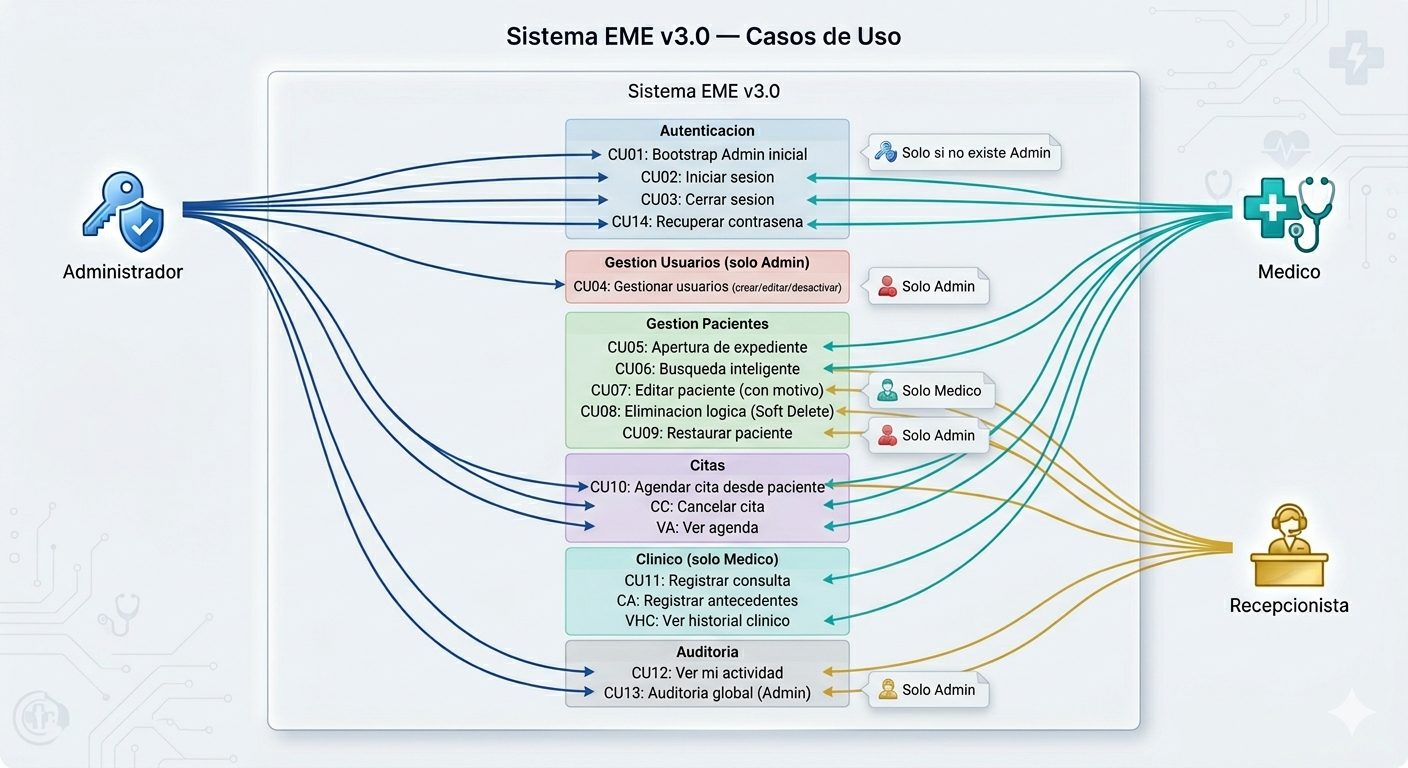
\includegraphics[width=0.8\textwidth]{img/Diagrama_Casos_Uso.png}
    \caption{Diagrama de Casos de Uso}
    \label{Diagrama de Casos de Uso}
\end{figure}

\subsection{Diagrama de Secuencia: Nuevo Paciente y Agendamiento}

Detalla el flujo completo desde la búsqueda previa del paciente en el hub, su creación mediante el modal unificado y el agendamiento inmediato de su primera cita con el paciente preseleccionado.

\begin{figure}[h]
    \centering
    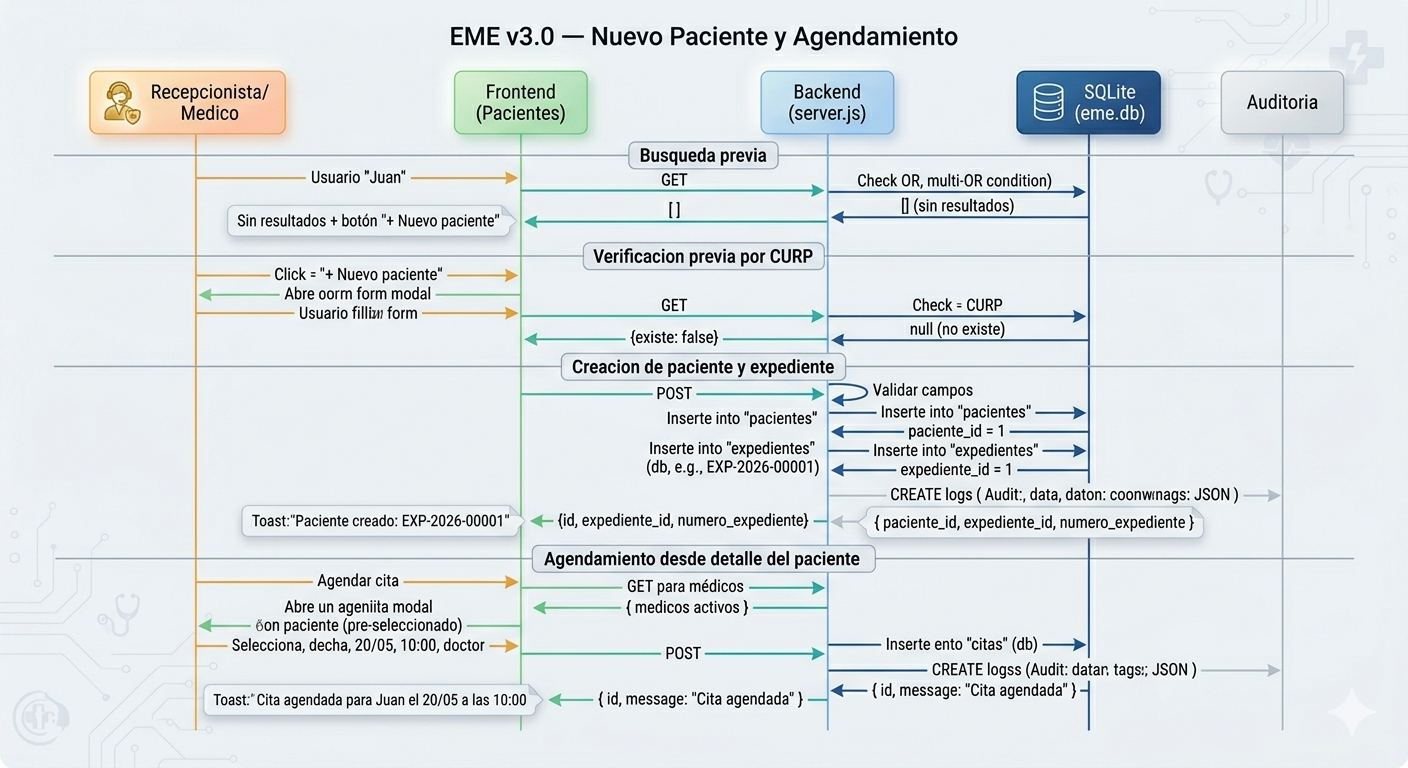
\includegraphics[width=0.8\textwidth]{img/Nuevo_Paciente_Agendamiento.png}
    \caption{Diagrama de Secuencia: Nuevo Paciente y Agendamiento de Cita}
    \label{Diagrama de Secuencia}
\end{figure}

\subsection{Diagrama de Actividad: Autenticación con Seguridad}

Representa el flujo completo de autenticación incluyendo las medidas de seguridad implementadas: verificación de rate limiting (5 intentos / 15 minutos), validación de credenciales con mensajes genéricos, almacenamiento en \texttt{sessionStorage}, inicio del monitor de inactividad de 15 minutos, aviso previo de 60 segundos y logout automático.

\begin{figure}[h]
    \centering
    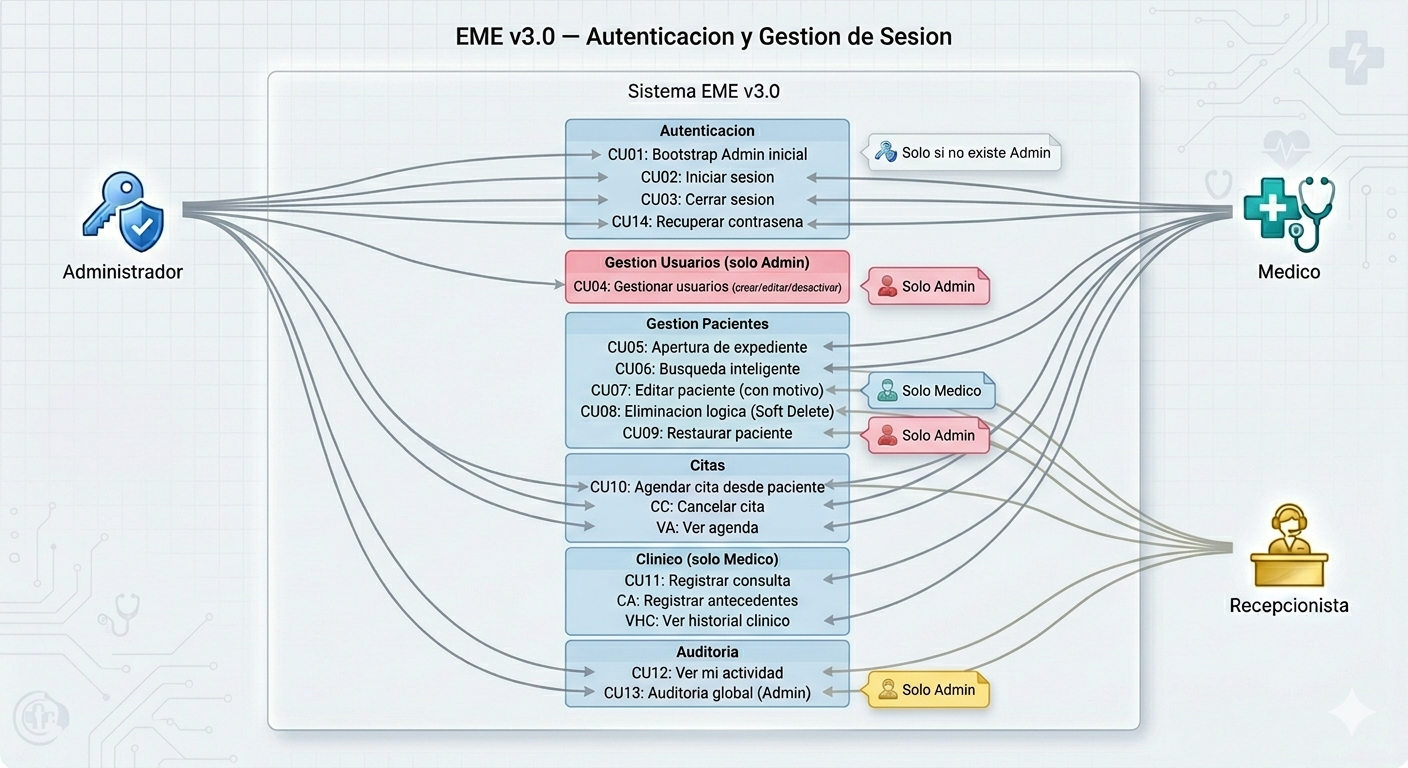
\includegraphics[width=0.8\textwidth]{img/Autenticacion_Seguridad.png}
    \caption{Diagrama de Actividad: Autenticación y Gestión de Sesión}
    \label{Diagrama de Actividad}
\end{figure}

\subsection{Diagrama de Componentes}

Muestra la arquitectura por capas del sistema con la capa de seguridad explícita: Helmet.js (cabeceras HTTP), CORS restringido, Rate Limiter, middleware de autenticación JWT y RBAC. La función \texttt{registrarAuditoria()} se muestra como componente transversal que se invoca desde todos los módulos funcionales.

\begin{figure}[h]
    \centering
    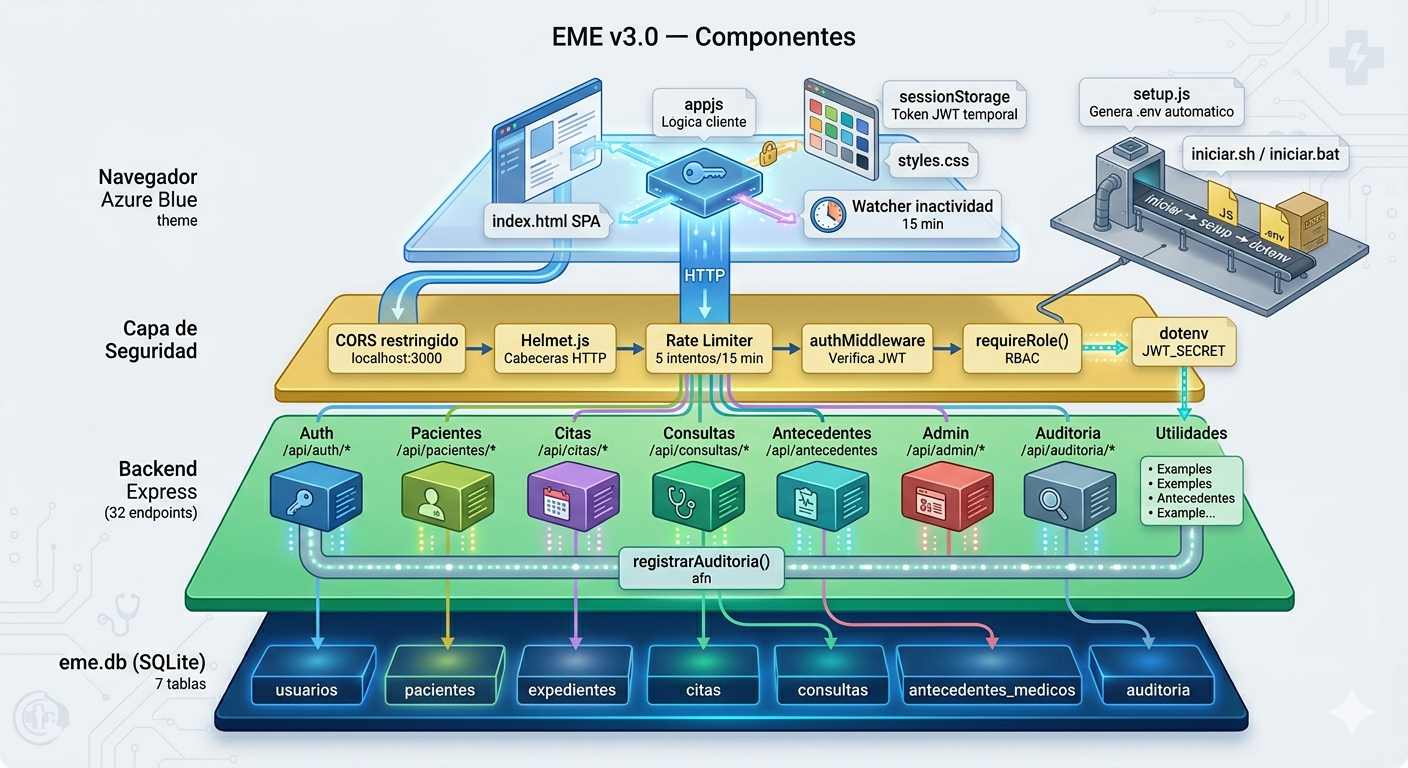
\includegraphics[width=0.8\textwidth]{img/Componentes.png}
    \caption{Diagrama de Componentes}
    \label{Diagrama de Componentes}
\end{figure}

\subsection{Diagrama de Clases}

Modelo orientado a objetos del dominio con las clases: Usuario (con roles admin / medico / recepcionista), Paciente (con campos de eliminación lógica), Expediente, Cita, Consulta, AntecedenteMedico y RegistroAuditoria. La clase Paciente incluye los métodos \texttt{eliminar()} (solo médico) y \texttt{restaurar()} (solo admin).

\begin{figure}[h]
    \centering
    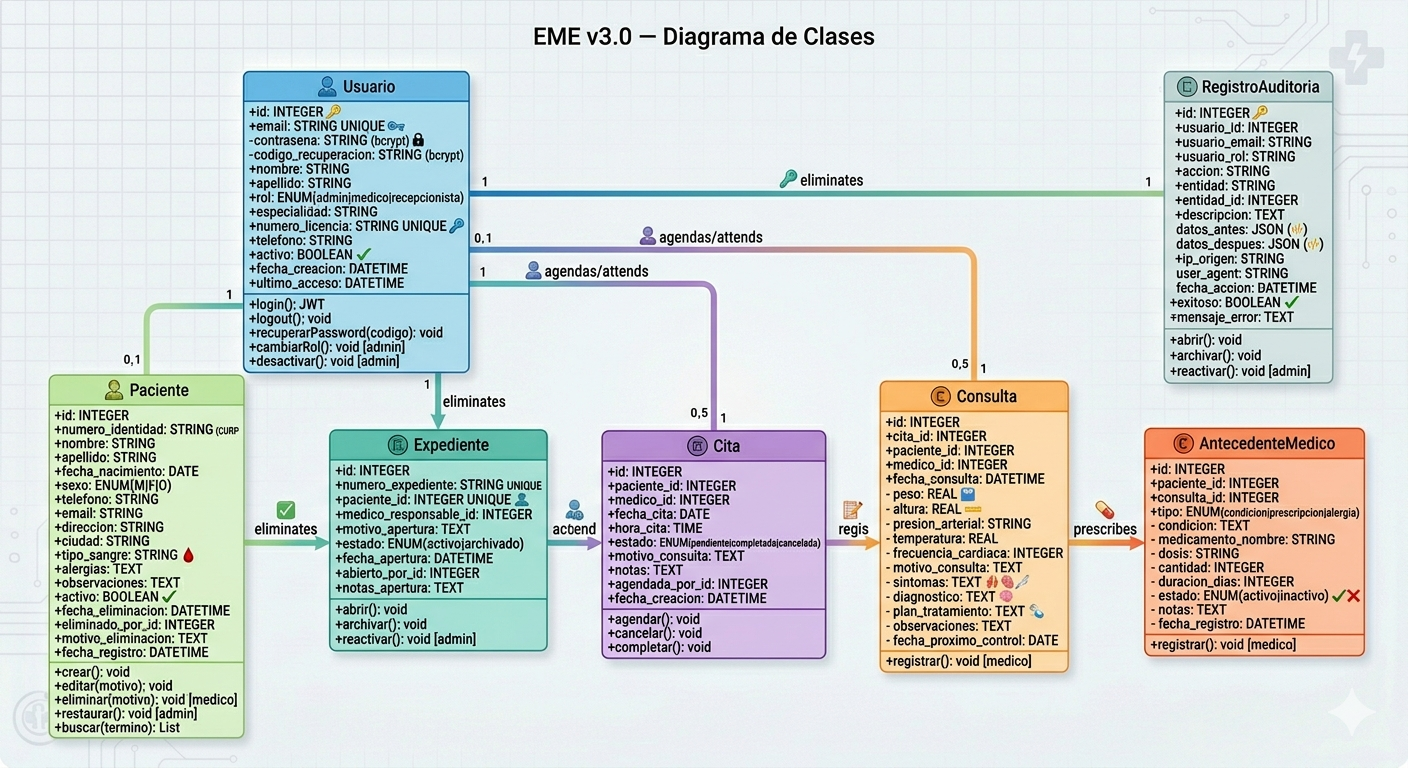
\includegraphics[width=0.8\textwidth]{img/Clases.png}
    \caption{Diagrama de Clases}
    \label{Diagrama de Clases}
\end{figure}

\subsection{Diagrama Entidad-Relación}

Esquema de la base de datos con 7 tablas activas: \texttt{usuarios}, \texttt{pacientes}, \texttt{expedientes}, \texttt{citas}, \texttt{consultas}, \texttt{antecedentes\_medicos} y \texttt{auditoria}. La tabla \texttt{pacientes} incluye los campos \texttt{activo}, \texttt{fecha\_eliminacion}, \texttt{eliminado\_por\_id} y \texttt{motivo\_eliminacion} para la eliminación lógica.

\begin{figure}[h]
    \centering
    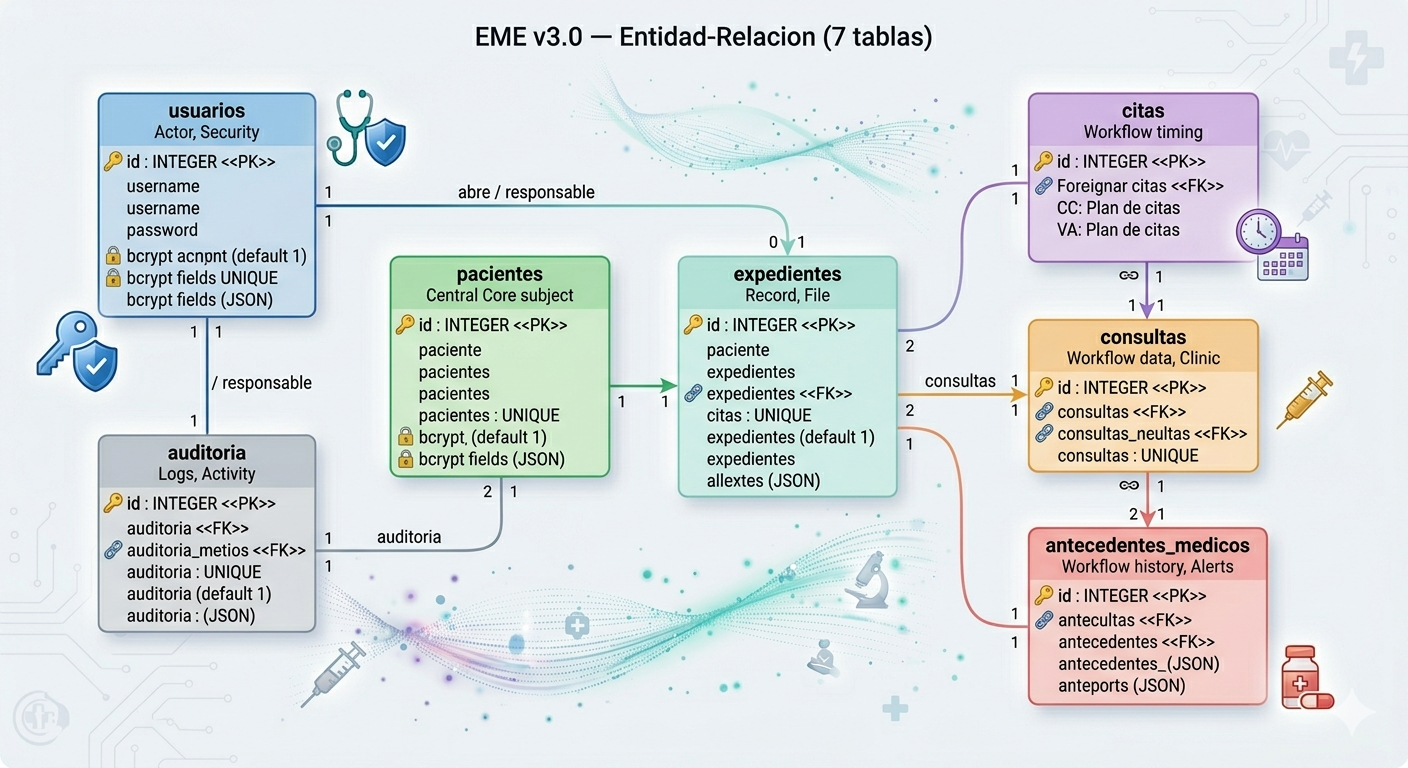
\includegraphics[width=0.8\textwidth]{img/Entidad_Relacion.png}
    \caption{Diagrama Entidad - Relación}
    \label{Diagrama Entidad - Relación}
\end{figure}

\subsection{Diagrama de Estados: Cita}

Estados posibles de una cita médica (pendiente, completada, cancelada) y las transiciones. Se documenta el comportamiento en cascada: cuando un médico elimina un paciente (soft delete), todas sus citas en estado \texttt{pendiente} se cancelan automáticamente.

\begin{figure}[h]
    \centering
    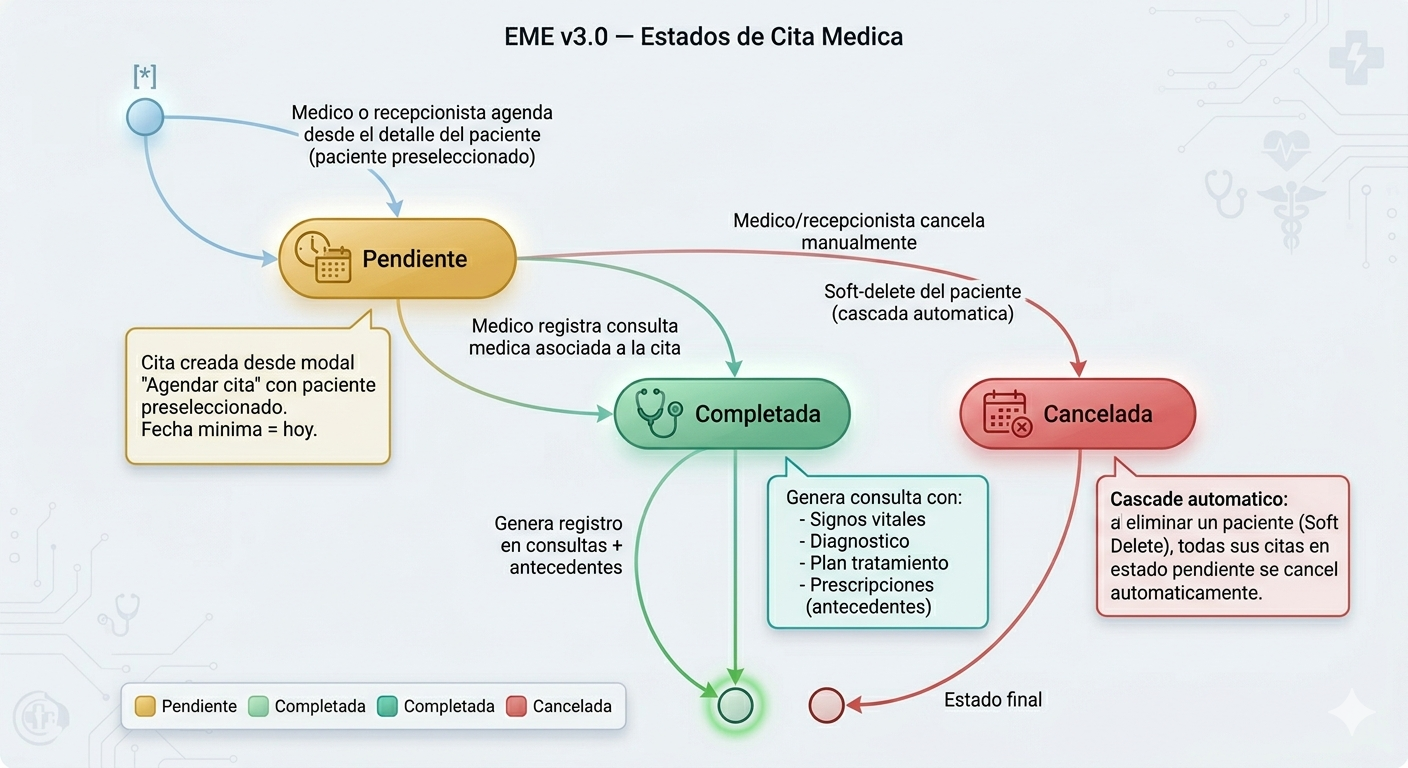
\includegraphics[width=0.8\textwidth]{img/Estados_Cita.png}
    \caption{Diagrama de Estados: Cita}
    \label{Diagrama de Estados}
\end{figure}

\subsection{Diagrama de Despliegue}

Topología del sistema en la computadora del consultorio. Incluye la capa de seguridad (Helmet, CORS, Rate Limiter), el servidor Node.js con Express, la base de datos SQLite y el navegador con \texttt{sessionStorage} y monitor de inactividad. Documenta que el archivo \texttt{.env} contiene el JWT\_SECRET y no se versiona en Git.

\begin{figure}[h]
    \centering
    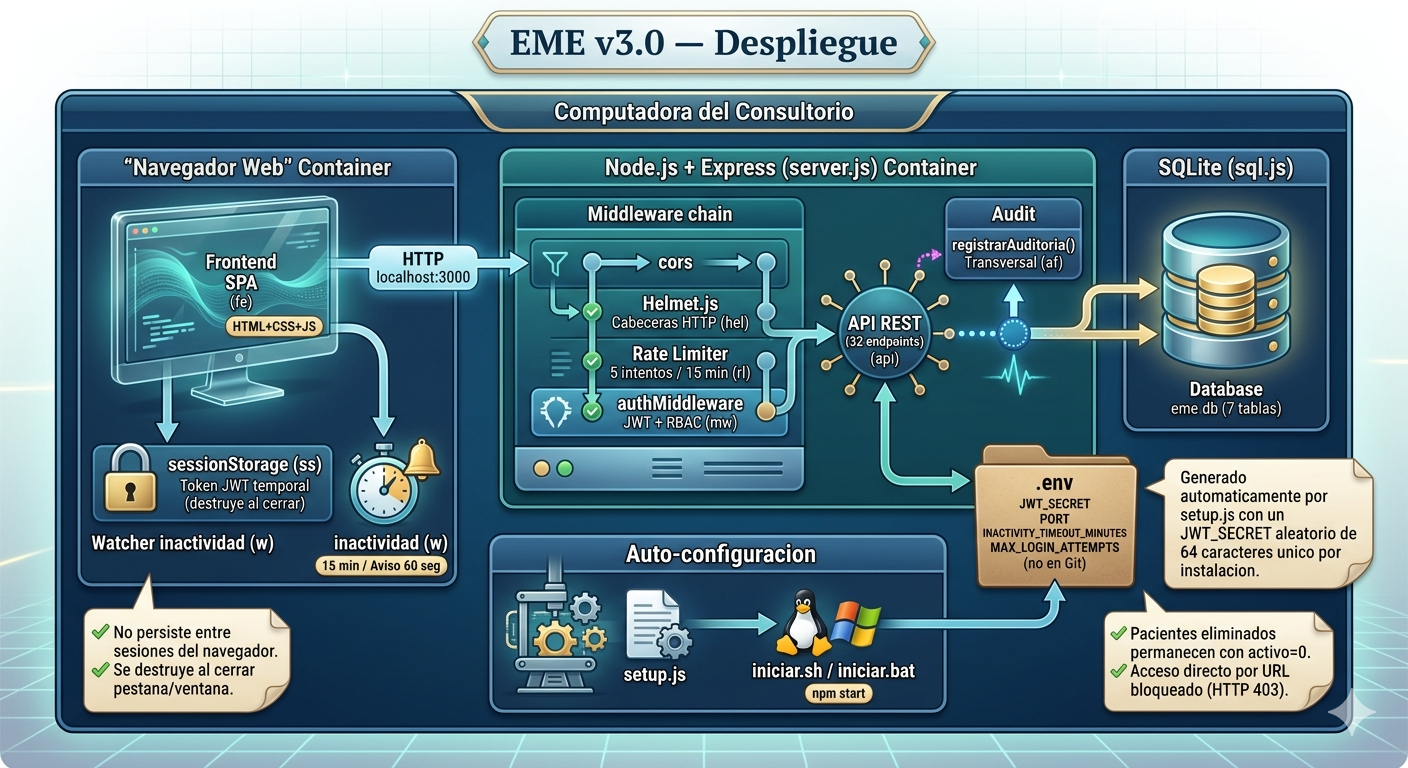
\includegraphics[width=0.8\textwidth]{img/Despliegue.png}
    \caption{Diagrama de Despliegue}
    \label{Diagrama de Despliegue}
\end{figure}

% ============================================================
% 8. MOCKUPS
% ============================================================
\section{Mockups}

A continuacion se muestran algunas de las interfaces clave que la versión final del sistema implementará. El sistema opera como SPA (Single Page Application) con navegación sin recarga.

\begin{figure}[H]
    \centering
    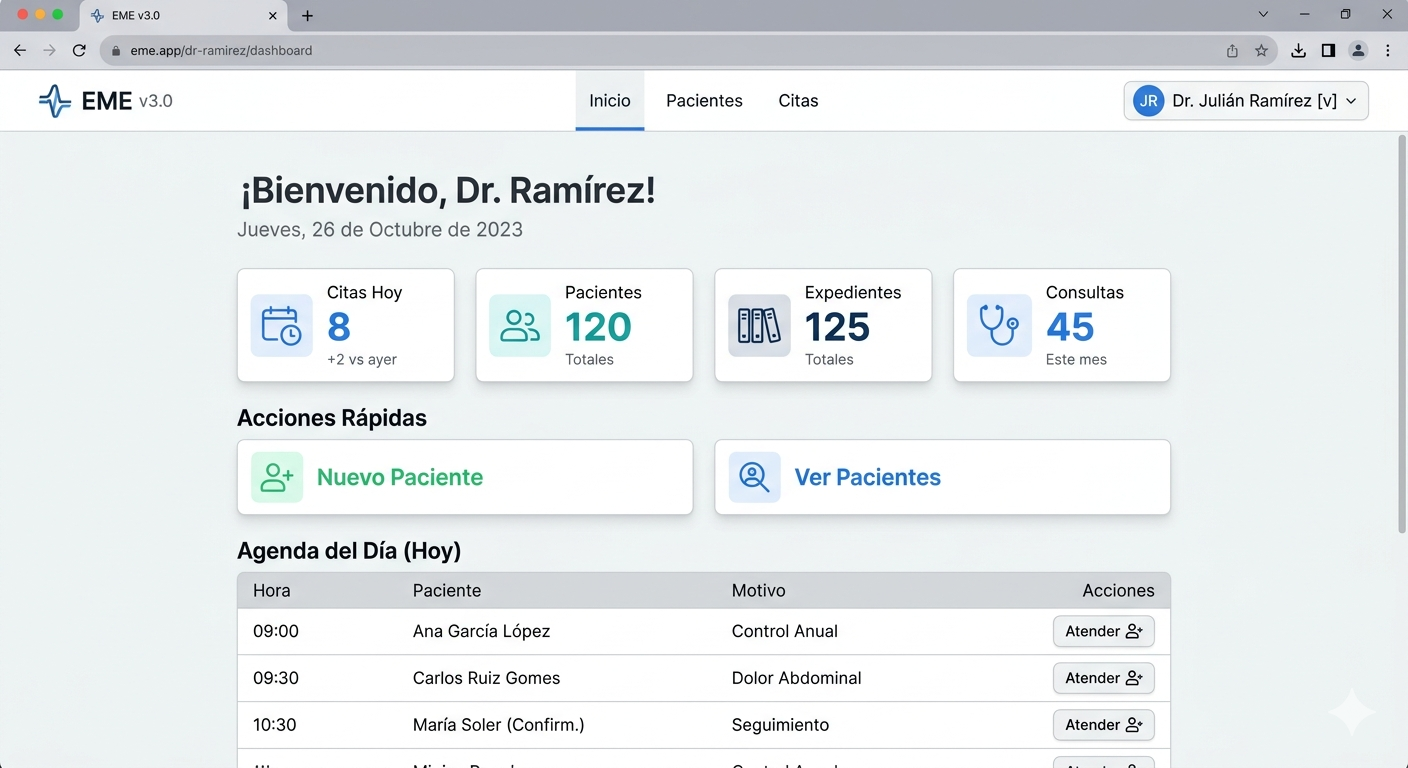
\includegraphics[width=1\textwidth]{img/Dashboard_Doctor.png}
    \caption{Dashboard del Médico}
    \label{Dashboard del Médico}
\end{figure}

\begin{figure}[H]
    \centering
    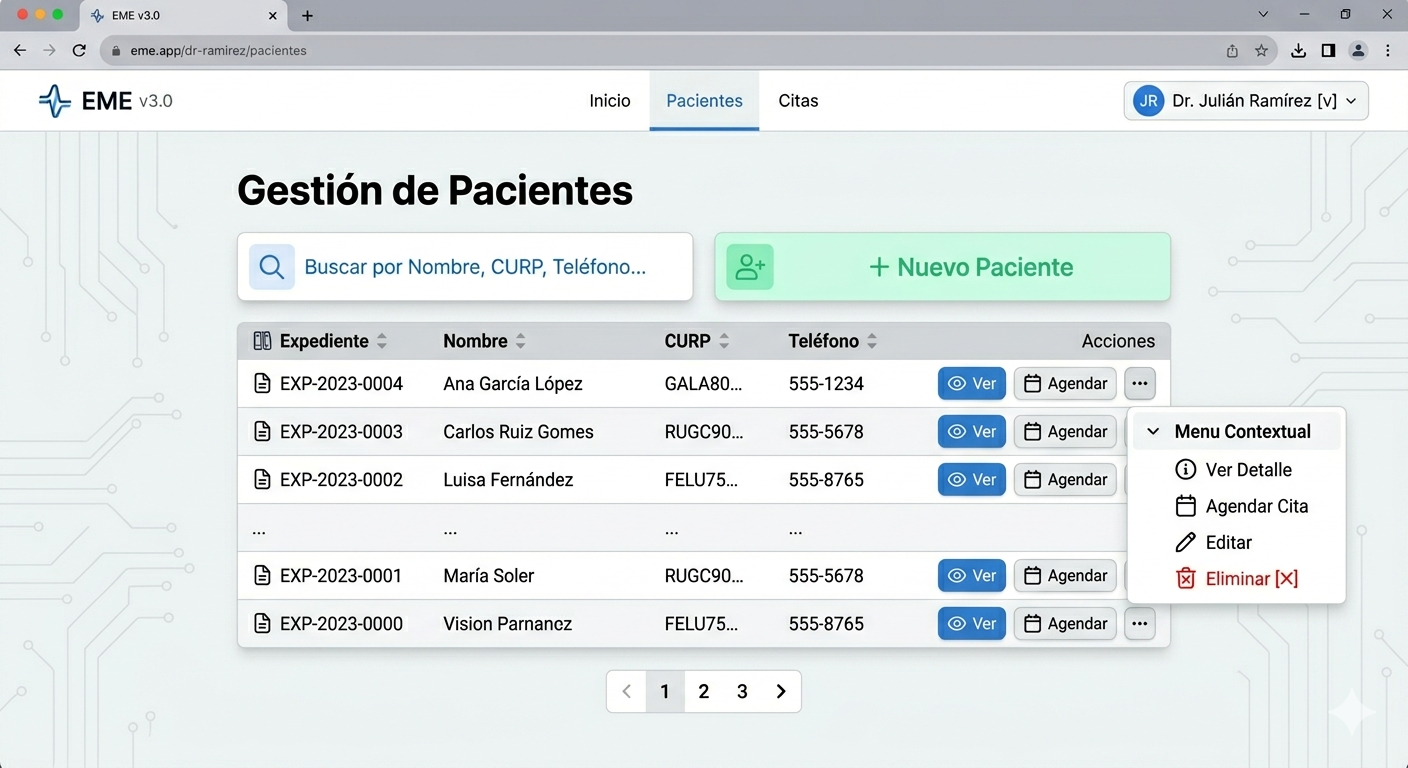
\includegraphics[width=1\textwidth]{img/Hub_Pacientes.png}
    \caption{Hub de Pacientes}
    \label{Hub de Pacientes}
\end{figure}

\begin{figure}[H]
    \centering
    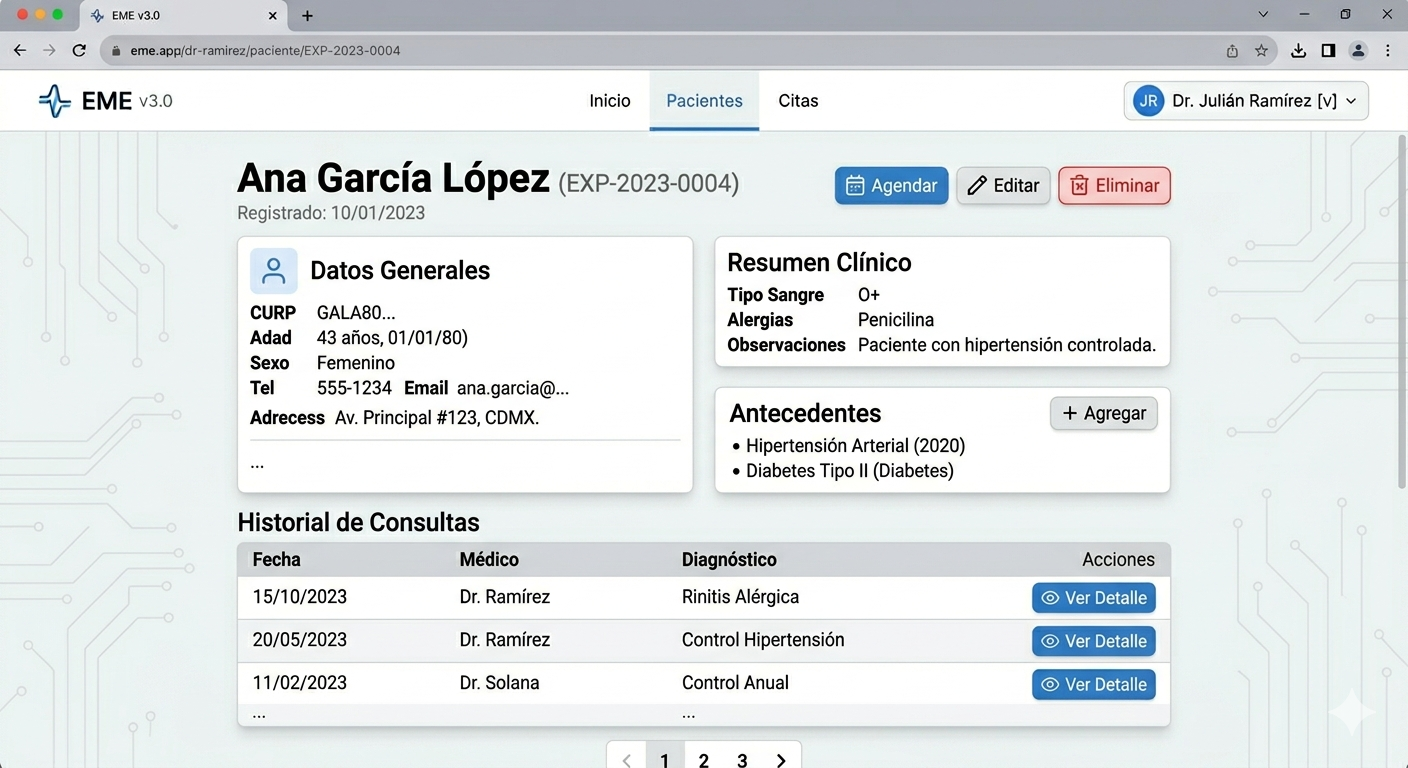
\includegraphics[width=1\textwidth]{img/Detalles_Paciente.png}
    \caption{Detalles del paciente}
    \label{Detalles del paciente}
\end{figure}

\begin{figure}[H]
    \centering
    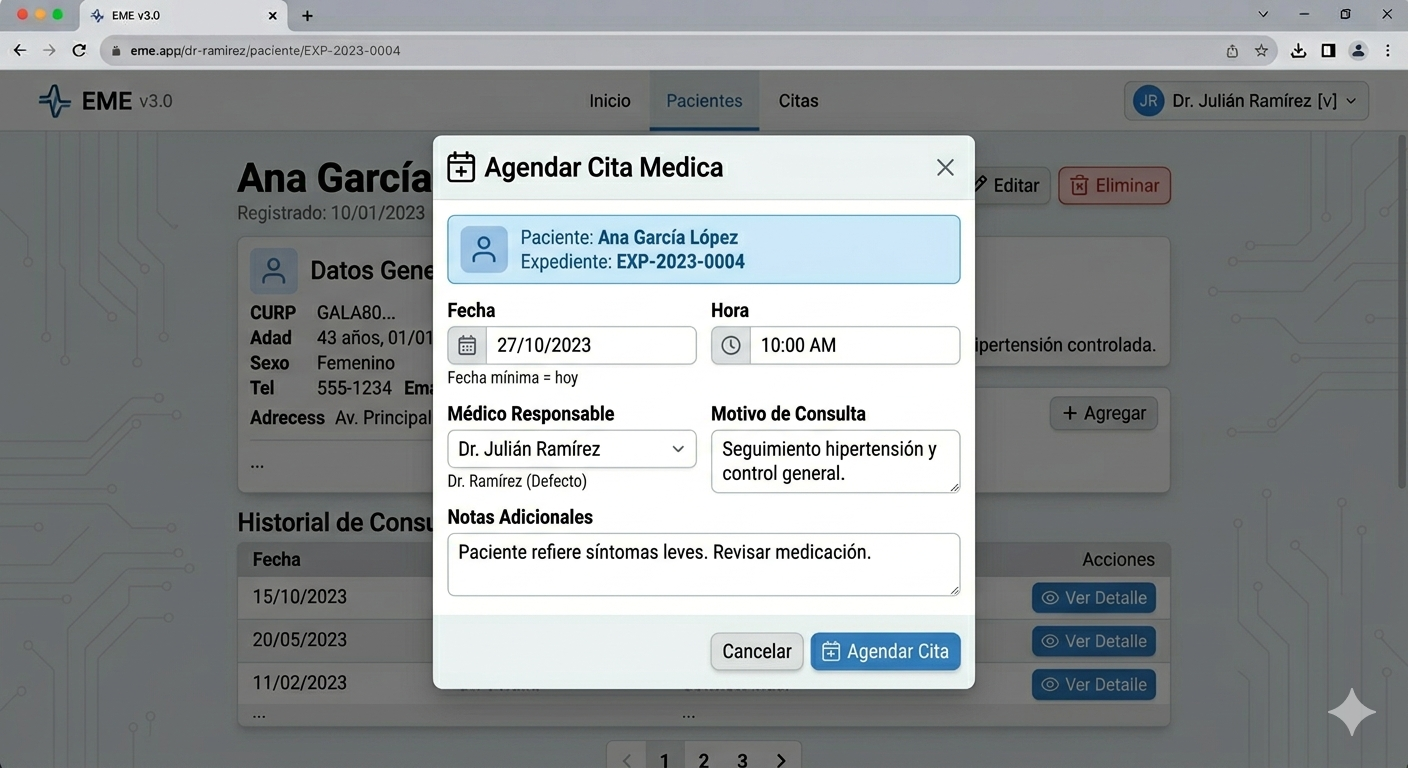
\includegraphics[width=1\textwidth]{img/Agendar_Cita.png}
    \caption{Modal Agendar Cita}
    \label{Agendar Cita}
\end{figure}

\begin{figure}[H]
    \centering
    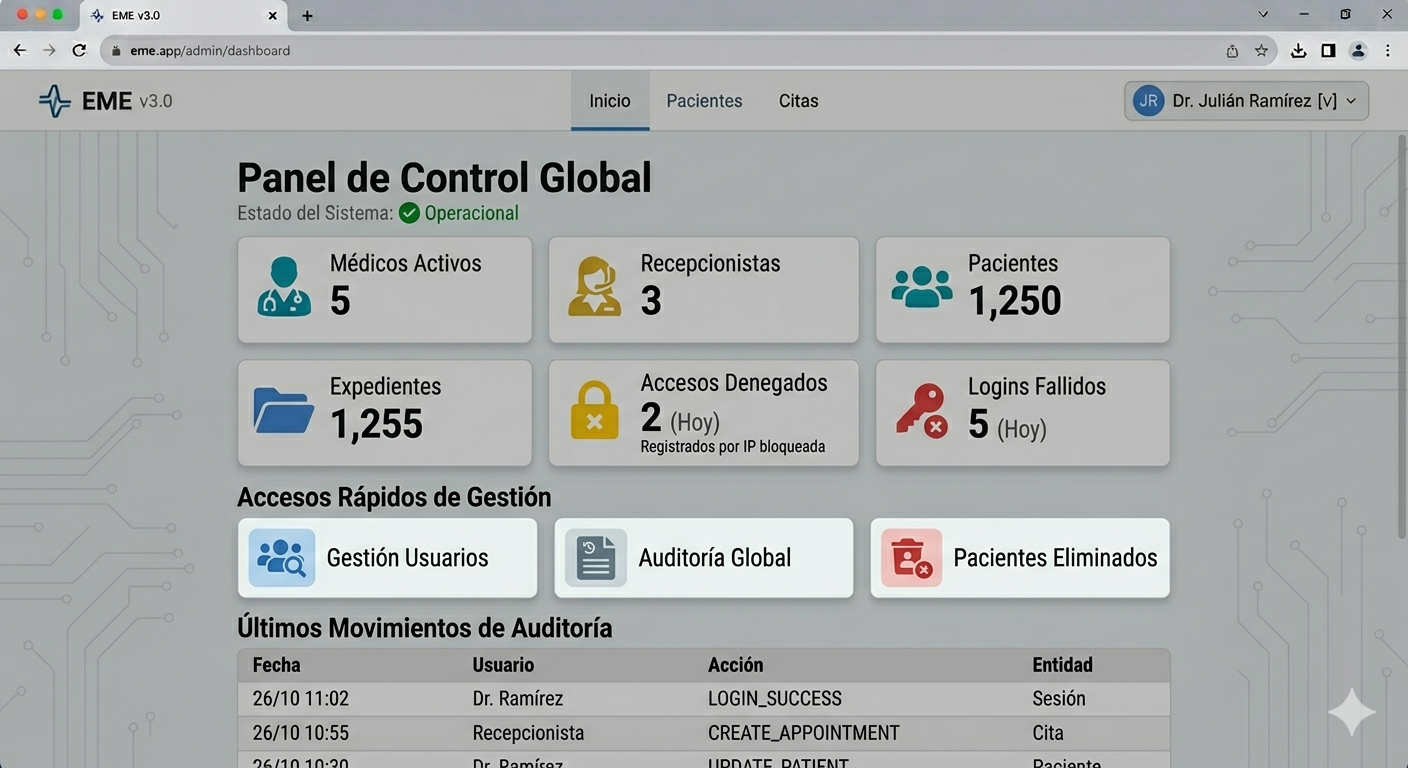
\includegraphics[width=1\textwidth]{img/Dashboard_Administrador.png}
    \caption{Dashboard del Administrador}
    \label{Dashboard del Administrador}
\end{figure}

\begin{figure}[H]
    \centering
    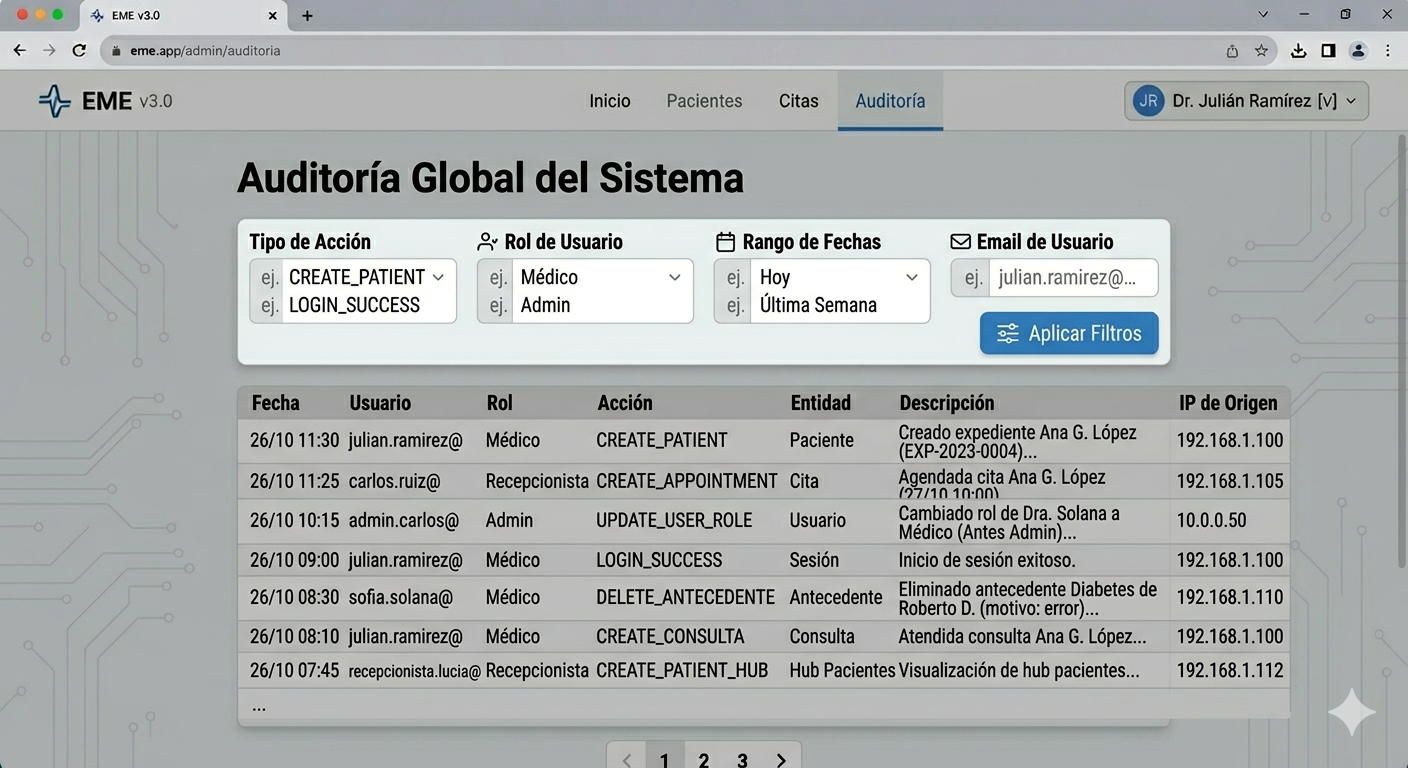
\includegraphics[width=1\textwidth]{img/Auditoria_Administrador.png}
    \caption{Auditoría del Administrador}
    \label{Auditoría del Administrador}
\end{figure}

\newpage

% ============================================================
% 9. CONCLUSIONES
% ============================================================
\section{Conclusiones}

El sistema de Expediente Médico Electrónico (EME) se desarrolló como un prototipo funcional completo que cubre el caso de uso de Apertura de Expediente Médico y se extiende para incluir la gestión integral del consultorio, conforme al estándar IEEE 830-1998. El sistema implementa los tres roles diferenciados (Administrador, Médico y Recepcionista), garantiza la confidencialidad de los datos clínicos mediante control de acceso basado en roles (RBAC) y proporciona trazabilidad completa mediante un registro de auditoría inmutable.

La evolución del sistema desde su versión inicial reflejó tres aprendizajes clave. Primero, la incorporación del rol Administrador resolvió la centralización de la gestión de cuentas y la separación de responsabilidades; el mecanismo de \textit{bootstrap} permitió que el primer usuario asumiera este rol sin requerir intervención técnica externa. Segundo, la implementación del hub de pacientes y el agendamiento centrado en el paciente eliminó el problema del dropdown masivo de pacientes y produjo una experiencia más natural alineada al flujo real del consultorio. Tercero, las medidas de hardening de seguridad (Helmet, rate limiting, sessionStorage, timeout de inactividad, .env auto-generado mediante \texttt{setup.js}) elevaron la calidad del prototipo a un nivel cercano al de producción.

Como áreas de mejora futura se identifican: la migración a una base de datos cliente-servidor (PostgreSQL o MySQL) para soportar concurrencia real; la incorporación de HTTPS mediante certificados Let's Encrypt; el desarrollo de una aplicación móvil complementaria; la integración con servicios de notificación por correo o SMS; y la implementación de firma digital certificada para las recetas electrónicas. El sistema queda estructurado de forma modular para facilitar estas extensiones sin reescritura mayor del código.

% ============================================================
% 10. REFERENCIAS
% ============================================================
\section{Referencias}

\begin{enumerate}
    \item IEEE Computer Society. (1998). \textit{IEEE Std 830-1998: IEEE Recommended Practice for Software Requirements Specifications}. Institute of Electrical and Electronics Engineers.
    \item Secretaría de Salud. (2012). \textit{NOM-024-SSA3-2012}. Norma Oficial Mexicana del Expediente Clínico Electrónico.
    \item OWASP Foundation. (2023). \textit{OWASP Top 10: 2021}. Recuperado de \url{https://owasp.org/Top10/}
    \item Helmet.js Team. (2024). \textit{Helmet --- Help secure Express apps with various HTTP headers}. Recuperado de \url{https://helmetjs.github.io/}
    \item Auth0 Inc. (2024). \textit{JSON Web Tokens --- jwt.io}. Recuperado de \url{https://jwt.io/introduction/}
    \item Mozilla Developer Network. (2024). \textit{Web Storage API: sessionStorage}. Recuperado de \url{https://developer.mozilla.org/en-US/docs/Web/API/Window/sessionStorage}
    \item Node.js Foundation. (2024). \textit{Node.js Documentation}. Recuperado de \url{https://nodejs.org/docs/}
    \item Express.js. (2024). \textit{Express --- Fast, unopinionated, minimalist web framework for Node.js}. Recuperado de \url{https://expressjs.com/}
\end{enumerate}

% ============================================================
% ANEXOS
% ============================================================
\newpage
\appendix

\section{Estructura del prototipo}

\begin{lstlisting}[language=bash]
eme-prototipo/
|-- server.js              Backend Node.js + Express (32 endpoints REST)
|-- setup.js               Auto-generador del archivo .env
|-- package.json           Dependencias del proyecto
|-- README.md              Documentacion de uso
|-- iniciar.sh             Script de inicio para Linux/macOS
|-- iniciar.bat            Script de inicio para Windows
|-- .env                   Variables de entorno (auto-generado, no en Git)
|-- .gitignore             Excluye .env, node_modules y eme.db
|-- eme.db                 Base de datos SQLite (auto-generada)
+-- public/
    |-- index.html         Frontend SPA con todas las pantallas
    |-- styles.css         Estilos visuales del sistema
    +-- app.js             Logica del cliente (sessionStorage, modales, timer)
\end{lstlisting}

\subsection*{Dependencias del proyecto}

\begin{itemize}
    \item \textbf{express} --- Servidor HTTP
    \item \textbf{bcryptjs} --- Hash de contraseñas (10 rondas)
    \item \textbf{jsonwebtoken} --- Generación y verificación de JWT
    \item \textbf{sql.js} --- SQLite en Node.js sin dependencias nativas
    \item \textbf{dotenv} --- Carga de variables de entorno desde \texttt{.env}
    \item \textbf{helmet} --- Cabeceras de seguridad HTTP automáticas
    \item \textbf{express-rate-limit} --- Rate limiting en endpoints de autenticación
    \item \textbf{cors} --- Control de orígenes permitidos
    \item \textbf{body-parser} --- Parseo de cuerpos JSON
\end{itemize}

\subsection*{Scripts de inicio}

\begin{itemize}
    \item \textbf{iniciar.sh} (Linux/macOS): Verifica Node.js, instala dependencias si no existen y ejecuta \texttt{npm start}.
    \item \textbf{iniciar.bat} (Windows): Equivalente para sistemas Windows.
    \item \textbf{setup.js}: Se ejecuta automáticamente antes del servidor (vía \texttt{npm start}). Genera el \texttt{.env} con un JWT\_SECRET aleatorio de 64 caracteres si no existe.
\end{itemize}

\section{Tabla de endpoints REST}

La siguiente tabla documenta los 32 endpoints de la API REST del sistema EME, con sus métodos HTTP, roles autorizados y descripción funcional.

\begin{longtable}{|L{1.3cm}|L{5.2cm}|L{2.5cm}|L{4cm}|}
    \hline
    \rowcolor{grisclaro}
    \textbf{Método} & \textbf{Endpoint}                            & \textbf{Roles}    & \textbf{Descripción}                      \\
    \hline
    \endfirsthead

    \hline
    \rowcolor{grisclaro}
    \textbf{Método} & \textbf{Endpoint}                            & \textbf{Roles}    & \textbf{Descripción}                      \\
    \hline
    \endhead

    \multicolumn{4}{|l|}{\cellcolor{grisclaro}\textbf{Autenticación (5)}}                                                          \\
    \hline
    GET             & \texttt{/api/auth/setup-status}              & Público           & Estado del sistema (¿requiere bootstrap?) \\
    \hline
    POST            & \texttt{/api/auth/registro}                  & Bootstrap / Admin & Registrar usuario                         \\
    \hline
    POST            & \texttt{/api/auth/login}                     & Público           & Iniciar sesión. Rate limit: 5/15 min      \\
    \hline
    POST            & \texttt{/api/auth/verificar-codigo}          & Público           & Verificar código de recuperación          \\
    \hline
    POST            & \texttt{/api/auth/reset-password}            & Público           & Restablecer contraseña                    \\
    \hline

    \multicolumn{4}{|l|}{\cellcolor{grisclaro}\textbf{Pacientes (8)}}                                                              \\
    \hline
    GET             & \texttt{/api/pacientes}                      & Médico, Recep.    & Listar pacientes activos                  \\
    \hline
    GET             & \texttt{/api/pacientes/buscar/:termino}      & Médico, Recep.    & Búsqueda inteligente (mín. 3 chars)       \\
    \hline
    GET             & \texttt{/api/pacientes/verificar/:identidad} & Médico, Recep.    & Verificar existencia por CURP             \\
    \hline
    GET             & \texttt{/api/pacientes/:id}                  & Médico, Recep.    & Detalle (filtrado por rol)                \\
    \hline
    POST            & \texttt{/api/pacientes}                      & Médico, Recep.    & Crear paciente sin expediente             \\
    \hline
    POST            & \texttt{/api/pacientes/apertura-expediente}  & Médico, Recep.    & Crear paciente + expediente               \\
    \hline
    PUT             & \texttt{/api/pacientes/:id}                  & Médico, Recep.    & Editar (motivo obligatorio)               \\
    \hline
    DELETE          & \texttt{/api/pacientes/:id}                  & Solo médico       & Eliminación lógica con cascada            \\
    \hline

    \multicolumn{4}{|l|}{\cellcolor{grisclaro}\textbf{Citas (5)}}                                                                  \\
    \hline
    GET             & \texttt{/api/citas}                          & Médico, Recep.    & Listar citas con filtros                  \\
    \hline
    GET             & \texttt{/api/citas/hoy}                      & Médico, Recep.    & Citas del día                             \\
    \hline
    POST            & \texttt{/api/citas}                          & Médico, Recep.    & Agendar cita                              \\
    \hline
    PUT             & \texttt{/api/citas/:id}                      & Médico, Recep.    & Cambiar estado de cita                    \\
    \hline
    DELETE          & \texttt{/api/citas/:id}                      & Médico, Recep.    & Cancelar cita                             \\
    \hline

    \multicolumn{4}{|l|}{\cellcolor{grisclaro}\textbf{Consultas y Antecedentes (3)}}                                               \\
    \hline
    POST            & \texttt{/api/consultas}                      & Solo médico       & Registrar consulta                        \\
    \hline
    GET             & \texttt{/api/consultas/:id}                  & Solo médico       & Detalle de consulta                       \\
    \hline
    POST            & \texttt{/api/antecedentes}                   & Solo médico       & Registrar antecedente o prescripción      \\
    \hline

    \multicolumn{4}{|l|}{\cellcolor{grisclaro}\textbf{Auditoría (2)}}                                                              \\
    \hline
    GET             & \texttt{/api/auditoria/mias}                 & Todos             & Auditoría propia (últimas 100)            \\
    \hline
    GET             & \texttt{/api/auditoria/todas}                & Solo admin        & Auditoría global con filtros              \\
    \hline

    \multicolumn{4}{|l|}{\cellcolor{grisclaro}\textbf{Administración (6, solo Admin)}}                                             \\
    \hline
    GET             & \texttt{/api/admin/usuarios}                 & Solo admin        & Listar todos los usuarios                 \\
    \hline
    PUT             & \texttt{/api/admin/usuarios/:id}             & Solo admin        & Editar datos de un usuario                \\
    \hline
    PUT             & \texttt{/api/admin/usuarios/:id/estado}      & Solo admin        & Activar/desactivar usuario                \\
    \hline
    GET             & \texttt{/api/admin/pacientes-eliminados}     & Solo admin        & Listar pacientes con activo=0             \\
    \hline
    POST            & \texttt{/api/admin/pacientes/:id/restaurar}  & Solo admin        & Restaurar paciente eliminado              \\
    \hline
    GET             & \texttt{/api/admin/stats}                    & Solo admin        & Estadísticas globales                     \\
    \hline

    \multicolumn{4}{|l|}{\cellcolor{grisclaro}\textbf{Utilidades (3)}}                                                             \\
    \hline
    GET             & \texttt{/api/medicos}                        & Autenticado       & Listar médicos activos                    \\
    \hline
    GET             & \texttt{/api/dashboard/stats}                & Autenticado       & Estadísticas del dashboard                \\
    \hline
    GET             & \texttt{/api/usuario/info}                   & Autenticado       & Datos del usuario en sesión               \\
    \hline
\end{longtable}

\end{document}
